\documentclass[12pt,a4paper]{article}

\usepackage[T1]{fontenc}
\usepackage[utf8]{inputenc}
\usepackage{mathptmx}
\usepackage[top=2.5cm,bottom=2.5cm,left=2.5cm,right=2.5cm]{geometry}
\usepackage{setspace}
\usepackage{graphicx}
\usepackage{booktabs}
\usepackage{array}
\usepackage{float}
\usepackage{caption}
\usepackage{listings}
\usepackage[hidelinks,hypertexnames=false]{hyperref}

\graphicspath{{figures/}}
\makeatletter
\setlength{\@fptop}{0pt}
\makeatother
\onehalfspacing
\setlength{\parindent}{0pt}
\setlength{\parskip}{6pt}
\captionsetup{font=small}
\lstset{basicstyle=\small\ttfamily,frame=single,columns=fullflexible,keepspaces=true}

\newcommand{\refDezan}{[1]}
\newcommand{\refAbramovici}{[2]}
\newcommand{\refVerilog}{[3]}
\newcommand{\refGamma}{[4]}
\newcommand{\refBlaha}{[5]}
\newcommand{\refMano}{[6]}
\newcommand{\refSugiyama}{[7]}
\newcommand{\refFowler}{[8]}
\newcommand{\refUML}{[9]}
\newcommand{\refTeaVM}{[10]}
\newcommand{\refJaCoCo}{[11]}
\newcommand{\refMermaid}{[12]}
\newcommand{\refGTKWave}{[13]}
\newcommand{\refRepository}{[14]}
\newcommand{\refHosted}{[15]}

\newcommand{\printreferences}{
[1] C. Dezan, L. Lagadec, B. Pottier; Object oriented approach for modeling digital circuits; Proceedings 1999 IEEE International Conference on Microelectronic Systems Education (MSE'99); Arlington, VA, USA; 1999, pp. 51-52.

[2] M. Abramovici, M. A. Breuer, A. D. Friedman; Digital Systems Testing and Testable Design; IEEE Press; New York, USA; 1st Edition, 1994, 672 pp.

[3] IEEE Computer Society; IEEE Standard for Verilog Hardware Description Language, IEEE Std 1364-2005; IEEE; New York, USA; 2006, 590 pp.

[4] E. Gamma, R. Helm, R. Johnson, J. Vlissides; Design Patterns, Elements of Reusable Object-Oriented Software; Addison-Wesley; Reading, MA, USA; 1st Edition, 1995, 395 pp.

[5] M. Blaha, J. Rumbaugh; Object-Oriented Modeling and Design with UML; Pearson Prentice Hall; Upper Saddle River, NJ, USA; 2nd Edition, 2005, 477 pp.

[6] M. M. Mano, M. D. Ciletti; Digital Design; Pearson; Chennai, India; 6th Edition, 2018, 765 pp.

[7] K. Sugiyama, S. Tagawa, M. Toda; Methods for visual understanding of hierarchical system structures; IEEE Transactions on Systems, Man, and Cybernetics; New York, USA; Volume 11: Number 2, 1981, pp. 109-125.
}

\newcommand{\printinternetsources}{
[8] M. Fowler; Inversion of Control Containers and the Dependency Injection pattern; 2004.\\ \url{https://martinfowler.com/articles/injection.html}

[9] Object Management Group; OMG Unified Modeling Language, Version 2.5.1; 2017.\\ \url{https://www.omg.org/spec/UML/2.5.1}

[10] TeaVM project; TeaVM, a Java bytecode to JavaScript compiler.\\ \url{https://teavm.org/}

[11] JaCoCo project; JaCoCo Java Code Coverage Library, Version 0.8.14.\\ \url{https://www.jacoco.org/jacoco/}

[12] Mermaid project; Mermaid, diagramming from text definitions.\\ \url{https://mermaid.js.org/}

[13] GTKWave project; GTKWave waveform viewer.\\ \url{https://gtkwave.sourceforge.net/}

[14] S. Rishab; Digital Circuit Simulator, project source code repository.\\ \url{https://github.com/MSRishab007/DigitalCircuitSimulator}

[15] S. Rishab; Digital Circuit Simulator, hosted browser version.\\ \url{https://msrishab007.github.io/DigitalCircuitSimulator/}
}


\begin{document}

\begin{titlepage}
\centering
\vspace*{1cm}

\includegraphics[width=4cm]{bits_logo.png}\par
\vspace{1cm}
{\Large\bfseries Birla Institute of Technology and Science, Pilani\par}
\vspace{2cm}
{\LARGE\bfseries Final Project Report\par}
\vspace{2.5cm}
\begin{tabular}{p{4.5cm}p{9.5cm}}
\toprule
\textbf{Area} & 25, Digital Electronics \\
\addlinespace
\textbf{Title of the Paper} & Object Oriented Approach for Modeling Digital Circuits \\
\addlinespace
\textbf{ID Number} & 2025H1030066P \\
\addlinespace
\textbf{Name} & S Rishab \\
\addlinespace
\textbf{Course Number} & SS G514 \\
\addlinespace
\textbf{Course Title} & Object Oriented Analysis and Design \\
\bottomrule
\end{tabular}
\vfill
{\large\bfseries Project Oct/Nov 2026\par}
\vspace*{1cm}
\end{titlepage}


\pagenumbering{roman}
\setcounter{page}{1}
\section*{Abstract}
\addcontentsline{toc}{section}{Abstract}

Digital circuits form the basis of computers and most modern electronic devices.
Building a physical prototype for each design change is slow and costly, so engineers test designs in software simulators before manufacture.
This project implements the circuit modeling part of the object-oriented approach proposed by Dezan, Lagadec, and Pottier as a simulator written in Java.
In this approach, software objects represent hardware elements such as logic gates and memory elements.

A user describes a circuit in a text file called a netlist.
The simulator calculates how the signals in the circuit change over time.
It presents the results as graphs called waveforms, as schematic diagrams, and as truth tables.
The system extends the original approach with signal delays, simulated hardware faults, timing analysis, and a measure of how many faults a test can detect.
It runs as a desktop application, a command line tool, and a browser application, and all three share one simulation engine.

An automated suite of 122 tests covers 91.3 percent of the source code lines outside the desktop interface.
This figure exceeds the 80 percent target that the project plan set for the domain logic and simulation engine.

\vspace{6pt}
\textbf{Keywords.} Digital circuit simulation, discrete-event simulation, object-oriented design, design patterns, fault injection.

\clearpage
\tableofcontents
\clearpage

\pagenumbering{arabic}
\setcounter{page}{1}
\section{Introduction}
\label{sec:introduction}

\subsection{Problem Statement}

A digital circuit processes information as electrical signals that take one of two values, written as 0 and 1.
Small components called logic gates combine these signals according to simple rules.
For example, a two-input AND gate produces 1 only when both of its inputs are 1.
Devices such as calculators and processors contain large numbers of these gates.

A design error in a manufactured circuit is expensive to correct, because the correction requires new hardware.
Engineers therefore check each design in software before building it.
A program that performs this check is a logic simulator.
It predicts how each signal in a circuit changes over time for a given set of inputs.

A physical gate takes a small amount of time to change its output, and this time is the propagation delay.
Delays can cause a circuit to produce incorrect values for a short period or to fail at high speed.
A simulator can reveal these effects only if it models time.
A simulator must also represent many kinds of components and allow developers to add new kinds.
Object-oriented design suits this need, because each software object can model one hardware element and hide its internal details from the others.

This project addresses the following problem.
The software receives a text description of a circuit built from logic gates and flip-flops.
A flip-flop is a memory element that stores one bit and updates it when a clock signal rises.
The software must calculate how signals travel through the circuit over simulated time.
It must reject any circuit that contains an invalid feedback loop.
Such a loop is a path from a gate output back to its own input with no flip-flop along the way.
It must also produce truth tables, timing estimates, and waveform output.

\subsection{Background Study}

\textbf{Digital circuit models.}
The output of a combinational circuit depends only on its present inputs \refMano{}.
A truth table describes such a circuit completely by listing the output for every input combination.
The output of a sequential circuit also depends on stored values, and these values form the state of the circuit.
A Mealy machine calculates its outputs from the inputs and the state, and a Moore machine calculates them from the state alone \refMano{}.
A clock signal controls when a synchronous sequential circuit updates its state.

\textbf{Discrete-event simulation.}
Most signals in a circuit remain unchanged for most of the time, so recalculating every gate at every instant wastes effort.
A discrete-event simulator acts only when a signal changes.
It stores each future change as an event in a priority queue, which is a data structure that always returns the earliest event first.
Each event may cause gates to produce further events after their propagation delays.
Simulated time therefore jumps directly from one event to the next.

\textbf{Fault modeling and waveform formats.}
Testing a circuit requires a way to describe what can go wrong in it.
The stuck-at model, which is a standard model in digital testing, assumes that a faulty wire holds the value 0 or 1 permanently \refAbramovici{}.
The fault coverage of a test is the percentage of modeled faults that the test can detect \refAbramovici{}.
Simulators commonly record their results as a waveform, which is a graph of each signal value against time.
The Value Change Dump (VCD) format, which the Verilog standard defines, stores these results as text that many viewing tools can read \refVerilog{}.

\textbf{Reference paper.}
Dezan, Lagadec, and Pottier describe a university course in which students build a logic simulator in the Smalltalk language \refDezan{}.
Their approach models combinational circuits as blocks of executable code and derives truth tables from these blocks.
It treats two circuits as equivalent when their truth tables match.
It models sequential circuits with separate transition and output functions in the Mealy or Moore style.
It builds larger circuits hierarchically, and nets carry the values that subcircuits exchange during simulation.
The authors also connect this model to placement and routing on field-programmable gate arrays, which are reconfigurable hardware chips.
The paper does not describe propagation delays, event scheduling, fault models, or timing analysis.
These topics form the main extensions in this project.

\textbf{Design patterns.}
A design pattern is a named and reusable solution to a recurring software design problem \refGamma{}.
Section~\ref{sec:patterns} describes the patterns that this system applies.

\subsection{Objectives and Contributions}

This project has two objectives.
The first objective is to implement the combinational, sequential, and hierarchical circuit models of the reference paper in Java.
The second objective is to extend these models with timing and fault analysis.
Section~\ref{sec:limitations} lists the parts of the reference paper that fall outside the scope of this project.
The list below states the main contributions of this project.

\begin{itemize}
\item The project provides a Java object model of wires, logic gates, tri-state buffers, flip-flops, clocks, and hierarchical modules.
\item The project provides a discrete-event engine with a separate delay for each component and four signal values. These values are 0, 1, X for an unknown value, and Z for a disconnected wire.
\item The project defines a netlist language that describes components, macros, Boolean functions, input stimuli, injected faults, and timed assertions.
\item The system generates truth tables and state tables, checks circuit equivalence, and reports stuck-at fault coverage. It also identifies the critical path, which is the slowest route through the circuit.
\item The system offers a desktop application, a command line tool, and a browser application over one shared engine. The graphical versions draw waveforms and schematic diagrams automatically.
\end{itemize}

\subsection{Requirements and Use Case Model}

Table~\ref{tab:requirements} lists the functional requirements of the system.
The first eight requirements come from the original project plan.
This project added requirements FR9 to FR15 during implementation.
FR9 and FR10 follow the truth table and equivalence methods of the reference paper, and FR11 to FR15 extend it.
Requirement FR5 has a specific scope in this implementation, because modules record the circuit hierarchy and the engine simulates the expanded gates.

\begin{table}[tbp]
\centering
\small
\caption{Functional requirements of the system}
\label{tab:requirements}
\begin{tabular}{l>{\raggedright\arraybackslash}p{8.8cm}ll}
\toprule
\textbf{ID} & \textbf{Requirement} & \textbf{Priority} & \textbf{Use Case} \\
\midrule
FR1 & The system shall parse a netlist file into an internal graph of circuit objects. & Must & UC-01 \\
FR2 & The system shall detect and reject combinational feedback loops. & Must & UC-02 \\
FR3 & The engine shall evaluate the Boolean logic of primitive gates. & Must & UC-03 \\
FR4 & The engine shall update flip-flops on the rising edge of their clock signal. & Must & UC-04 \\
FR5 & The system shall support reusable hierarchical modules built from gates. & Must & UC-05 \\
FR6 & The engine shall model propagation delays with a priority event queue. & Must & UC-06 \\
FR7 & The system should allow permanent stuck-at faults on chosen wires. & Should & UC-07 \\
FR8 & The system should export signal changes in a standard waveform format. & Should & UC-08 \\
FR9 & The system should generate truth tables and state tables. & Should & UC-09 \\
FR10 & The system should compare two circuits and report a differing input row. & Should & UC-10 \\
FR11 & The system should report the critical path and maximum clock frequency. & Should & UC-11 \\
FR12 & The system should report the stuck-at fault coverage of the input stimuli. & Should & UC-12 \\
FR13 & The system should draw a schematic diagram of the circuit automatically. & Should & UC-13 \\
FR14 & The system should check expected wire values and report each result. & Should & UC-14 \\
FR15 & The system should allow simulation to advance one event at a time. & Should & UC-15 \\
\bottomrule
\end{tabular}
\end{table}

The project plan also sets three non-functional requirements.
The event queue must process at least ten thousand events per second.
A new gate type must require only one new class in the component model.
Automated unit tests must cover at least 80 percent of the domain logic and simulation engine.
Section~\ref{sec:evaluation} reports the measured results for these requirements.

Figure~\ref{fig:usecase} presents the use case model.
A use case describes one service that the system provides to an external actor \refBlaha{}.
The primary actor is the electronics engineer, who writes a netlist and requests a simulation or an analysis.
The secondary actor is an external waveform viewer, which reads the exported VCD file.
An include relationship marks behavior that a use case always performs, and an extend relationship marks optional behavior.

\begin{figure}[H]
\centering
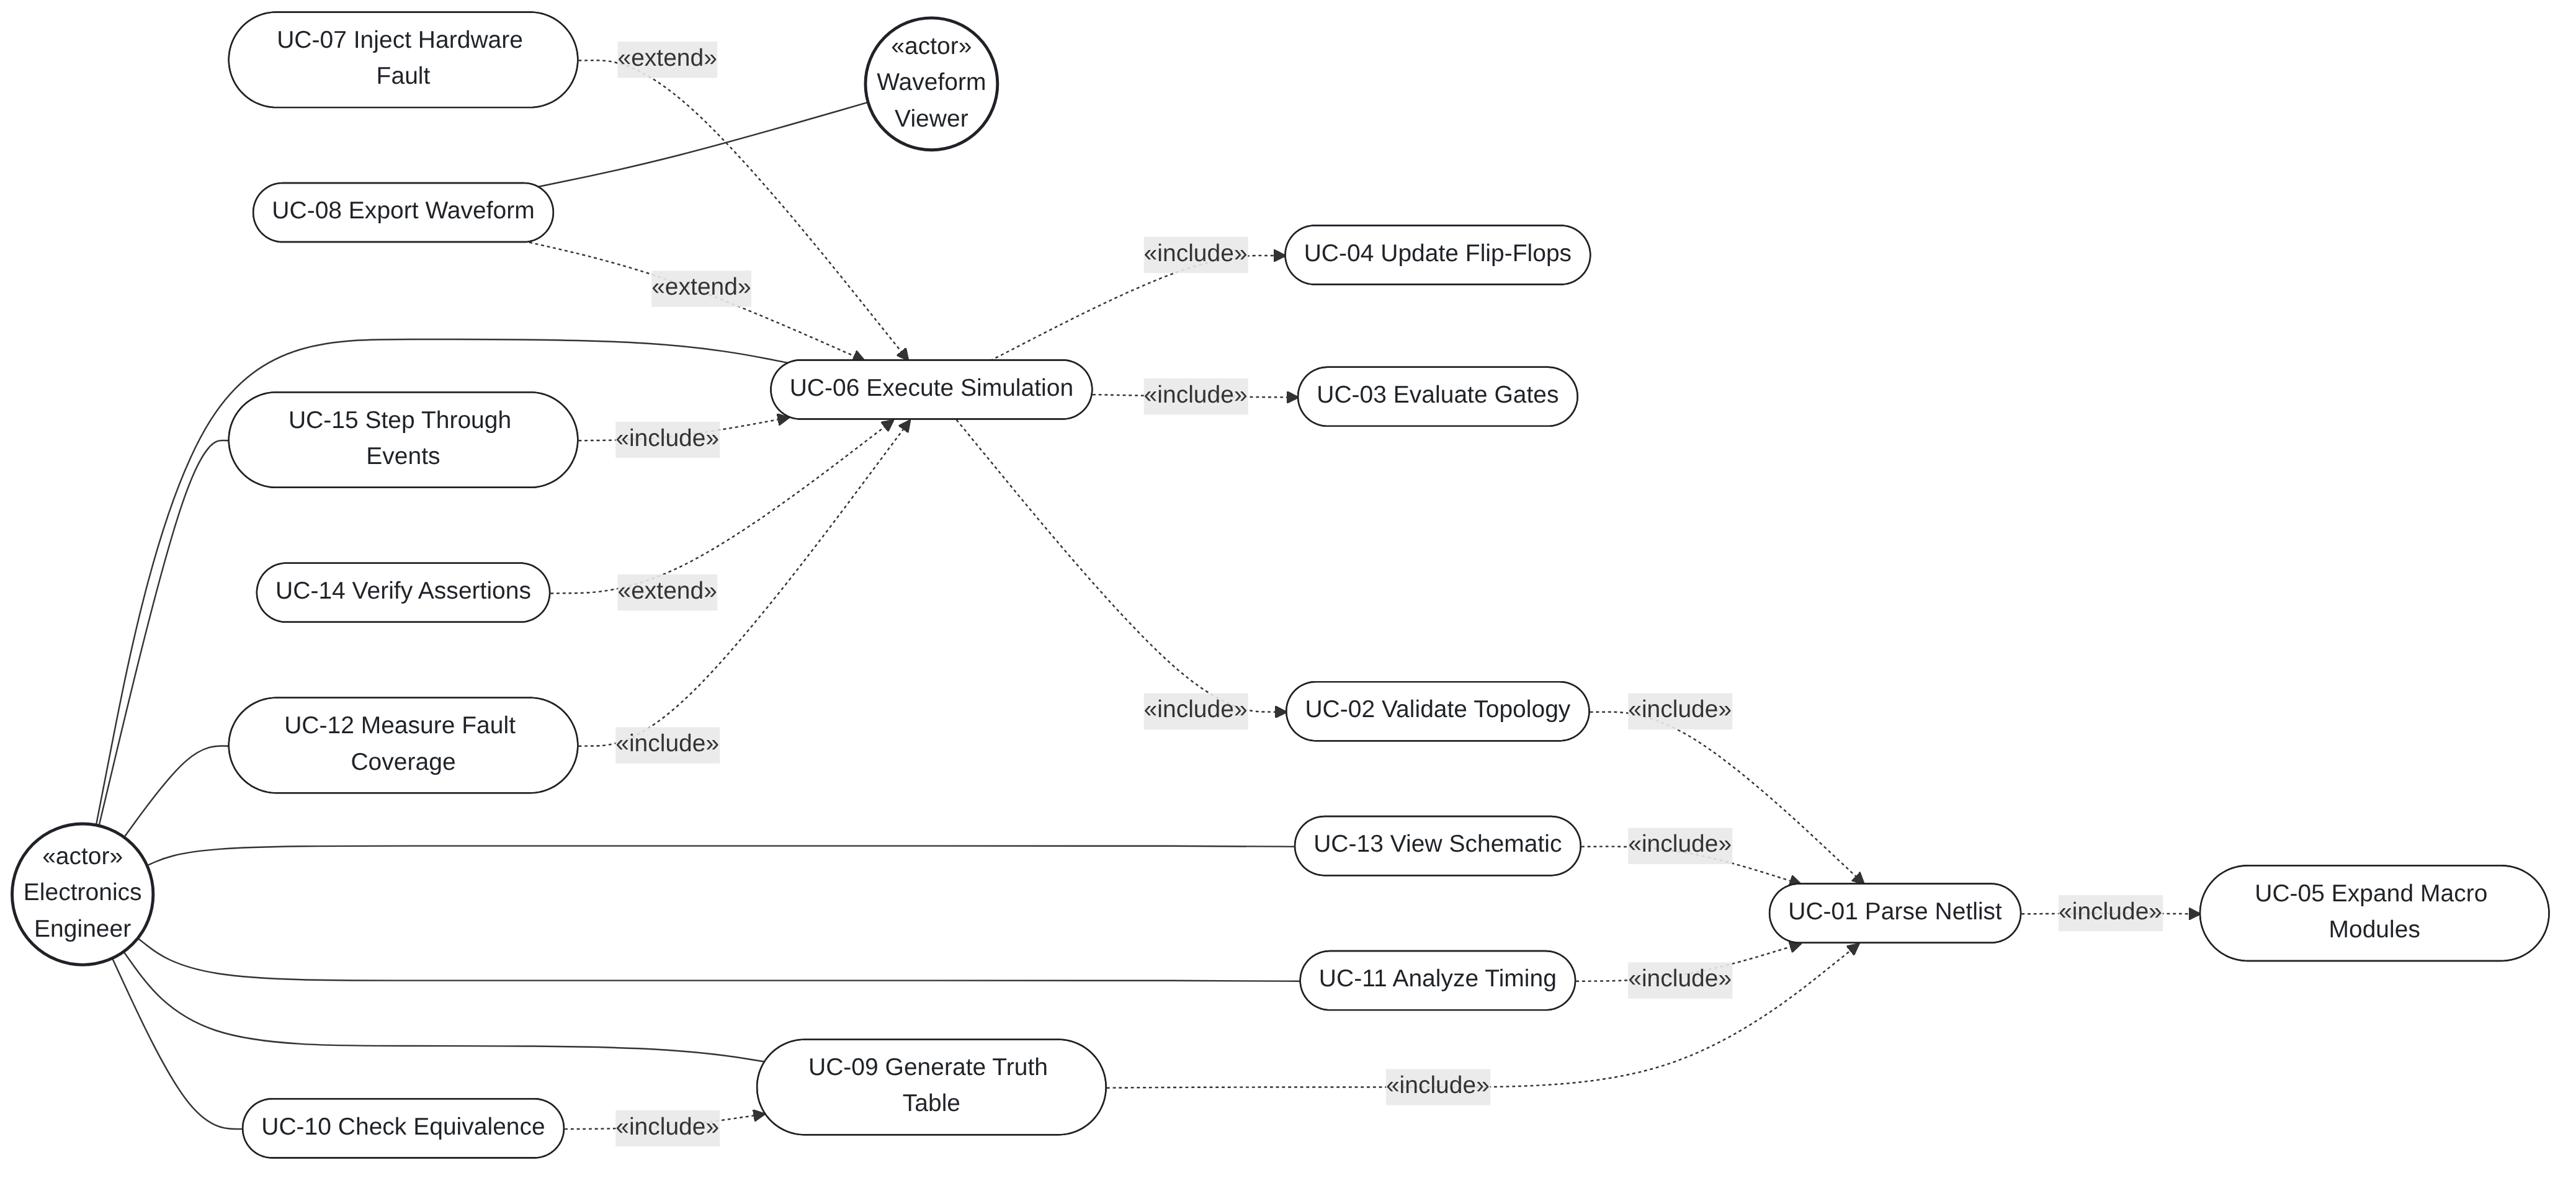
\includegraphics[width=\textwidth]{useCaseDiagram.png}
\caption{Use case diagram of the digital circuit simulator}
\label{fig:usecase}
\end{figure}

\section{Approach to the Solution}
\subsection{Development Methodology}
\subsection{Execution Pipeline}
\subsection{Testing Strategy}

\section{Use of Design Patterns}
\label{sec:patterns}
\subsection{Observer Pattern for Signal Propagation}
\subsection{Composite Pattern for Circuit Hierarchy}
\subsection{Factory Method Pattern for Component Creation}
\subsection{State Pattern for Memory Elements}
\subsection{Facade Pattern for Application Services}
\subsection{Dependency Injection in Place of the Planned Singleton}

\section{Design of the Solution}
\label{sec:design}

This section presents the design of the system in the Unified Modeling Language (UML) \refUML{}.
This project wrote all UML diagrams in the Mermaid text notation \refMermaid{}.

\subsection{System Architecture}

Figure~\ref{fig:architecture} presents the four layers of the system.
Each layer depends only on the layers below it.
The presentation layer contains the three user interfaces.
The application layer offers the operations that these interfaces share.
The parsing and analysis layer turns netlist text into objects and runs simulations and analyses.
The domain model layer represents the circuit itself.

The browser version reuses the Java layers without a server.
The TeaVM compiler \refTeaVM{} translates the Java engine to JavaScript.
The class \texttt{WasmBridge} exports functions that accept netlist text and return JSON, and the page \texttt{index.html} calls these functions and draws the results.

\begin{figure}[H]
\centering
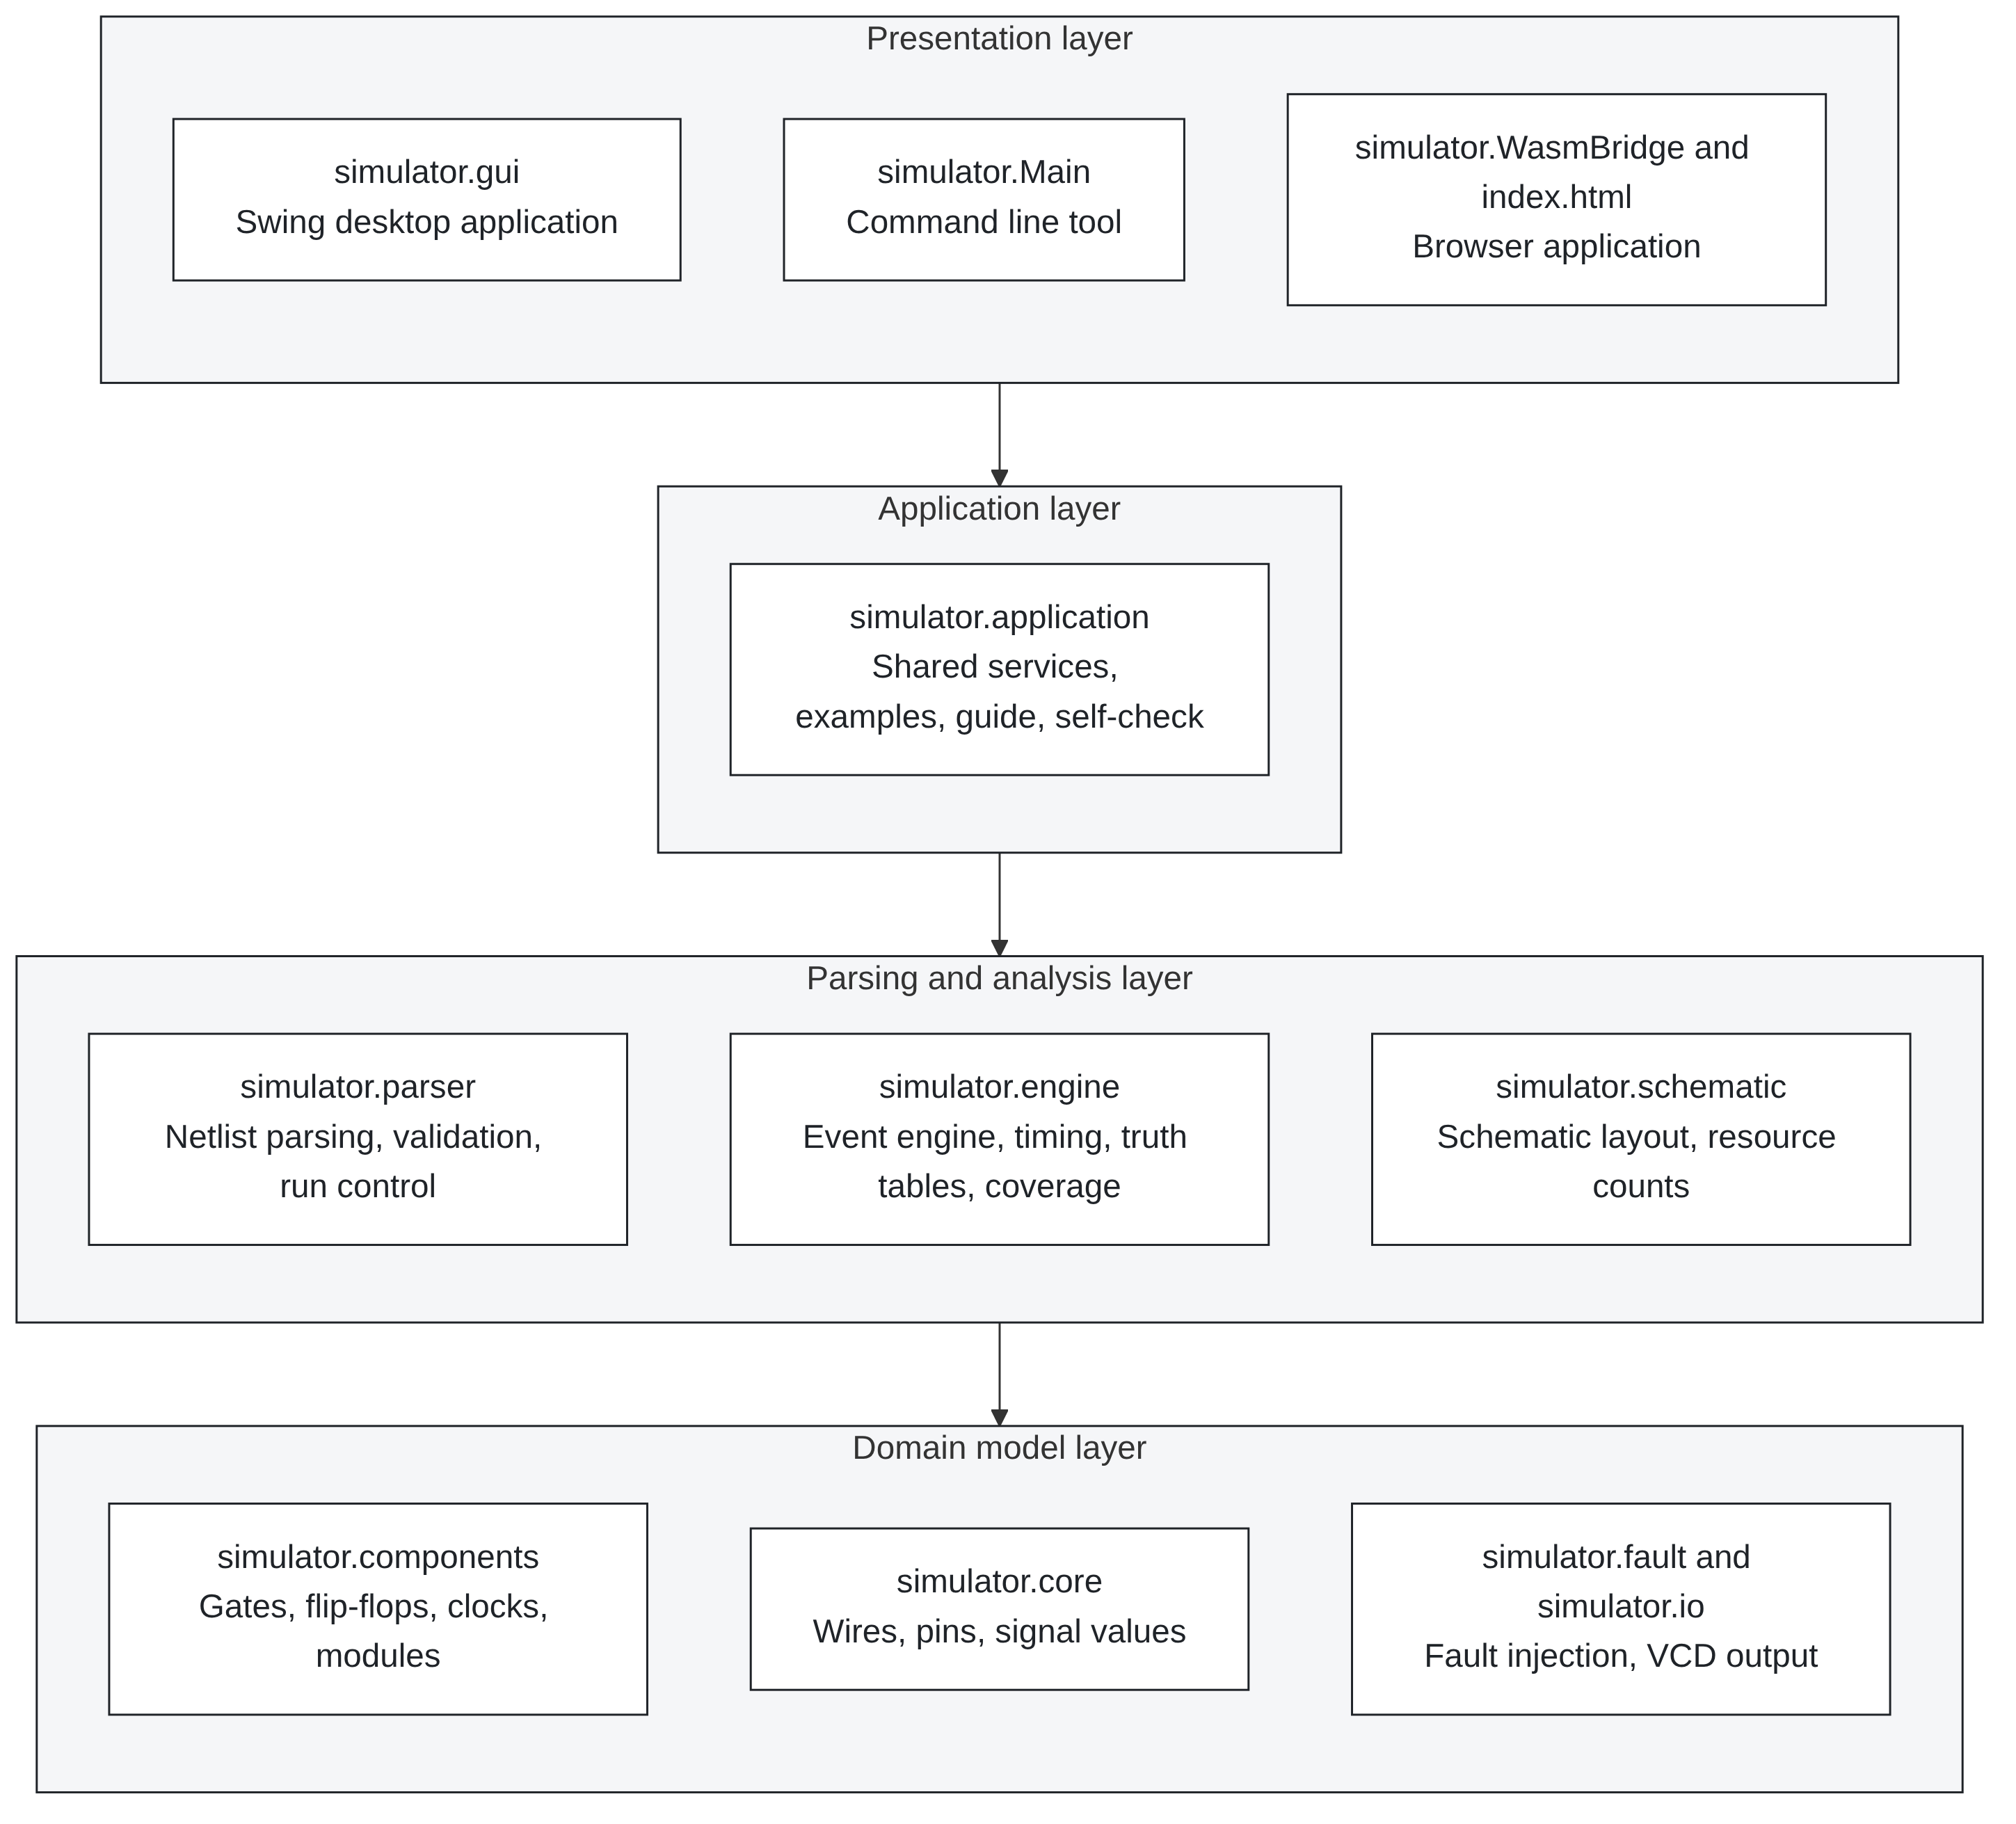
\includegraphics[width=0.9\textwidth]{architectureDiagram.png}
\caption{Layered architecture of the system}
\label{fig:architecture}
\end{figure}

\subsection{Class Model}

Figure~\ref{fig:classdomain} presents the domain model.
\texttt{DigitalComponent} is the abstract base class of every component and owns its pins.
\texttt{LogicGate} adds a propagation delay and schedules an event when its calculated output changes.
Each concrete gate implements only its own Boolean function.
The figure groups the seven simple gates into one box to save space.
A \texttt{Wire} connects output pins to input pins and resolves the values of its drivers into one value.

\begin{figure}[H]
\centering
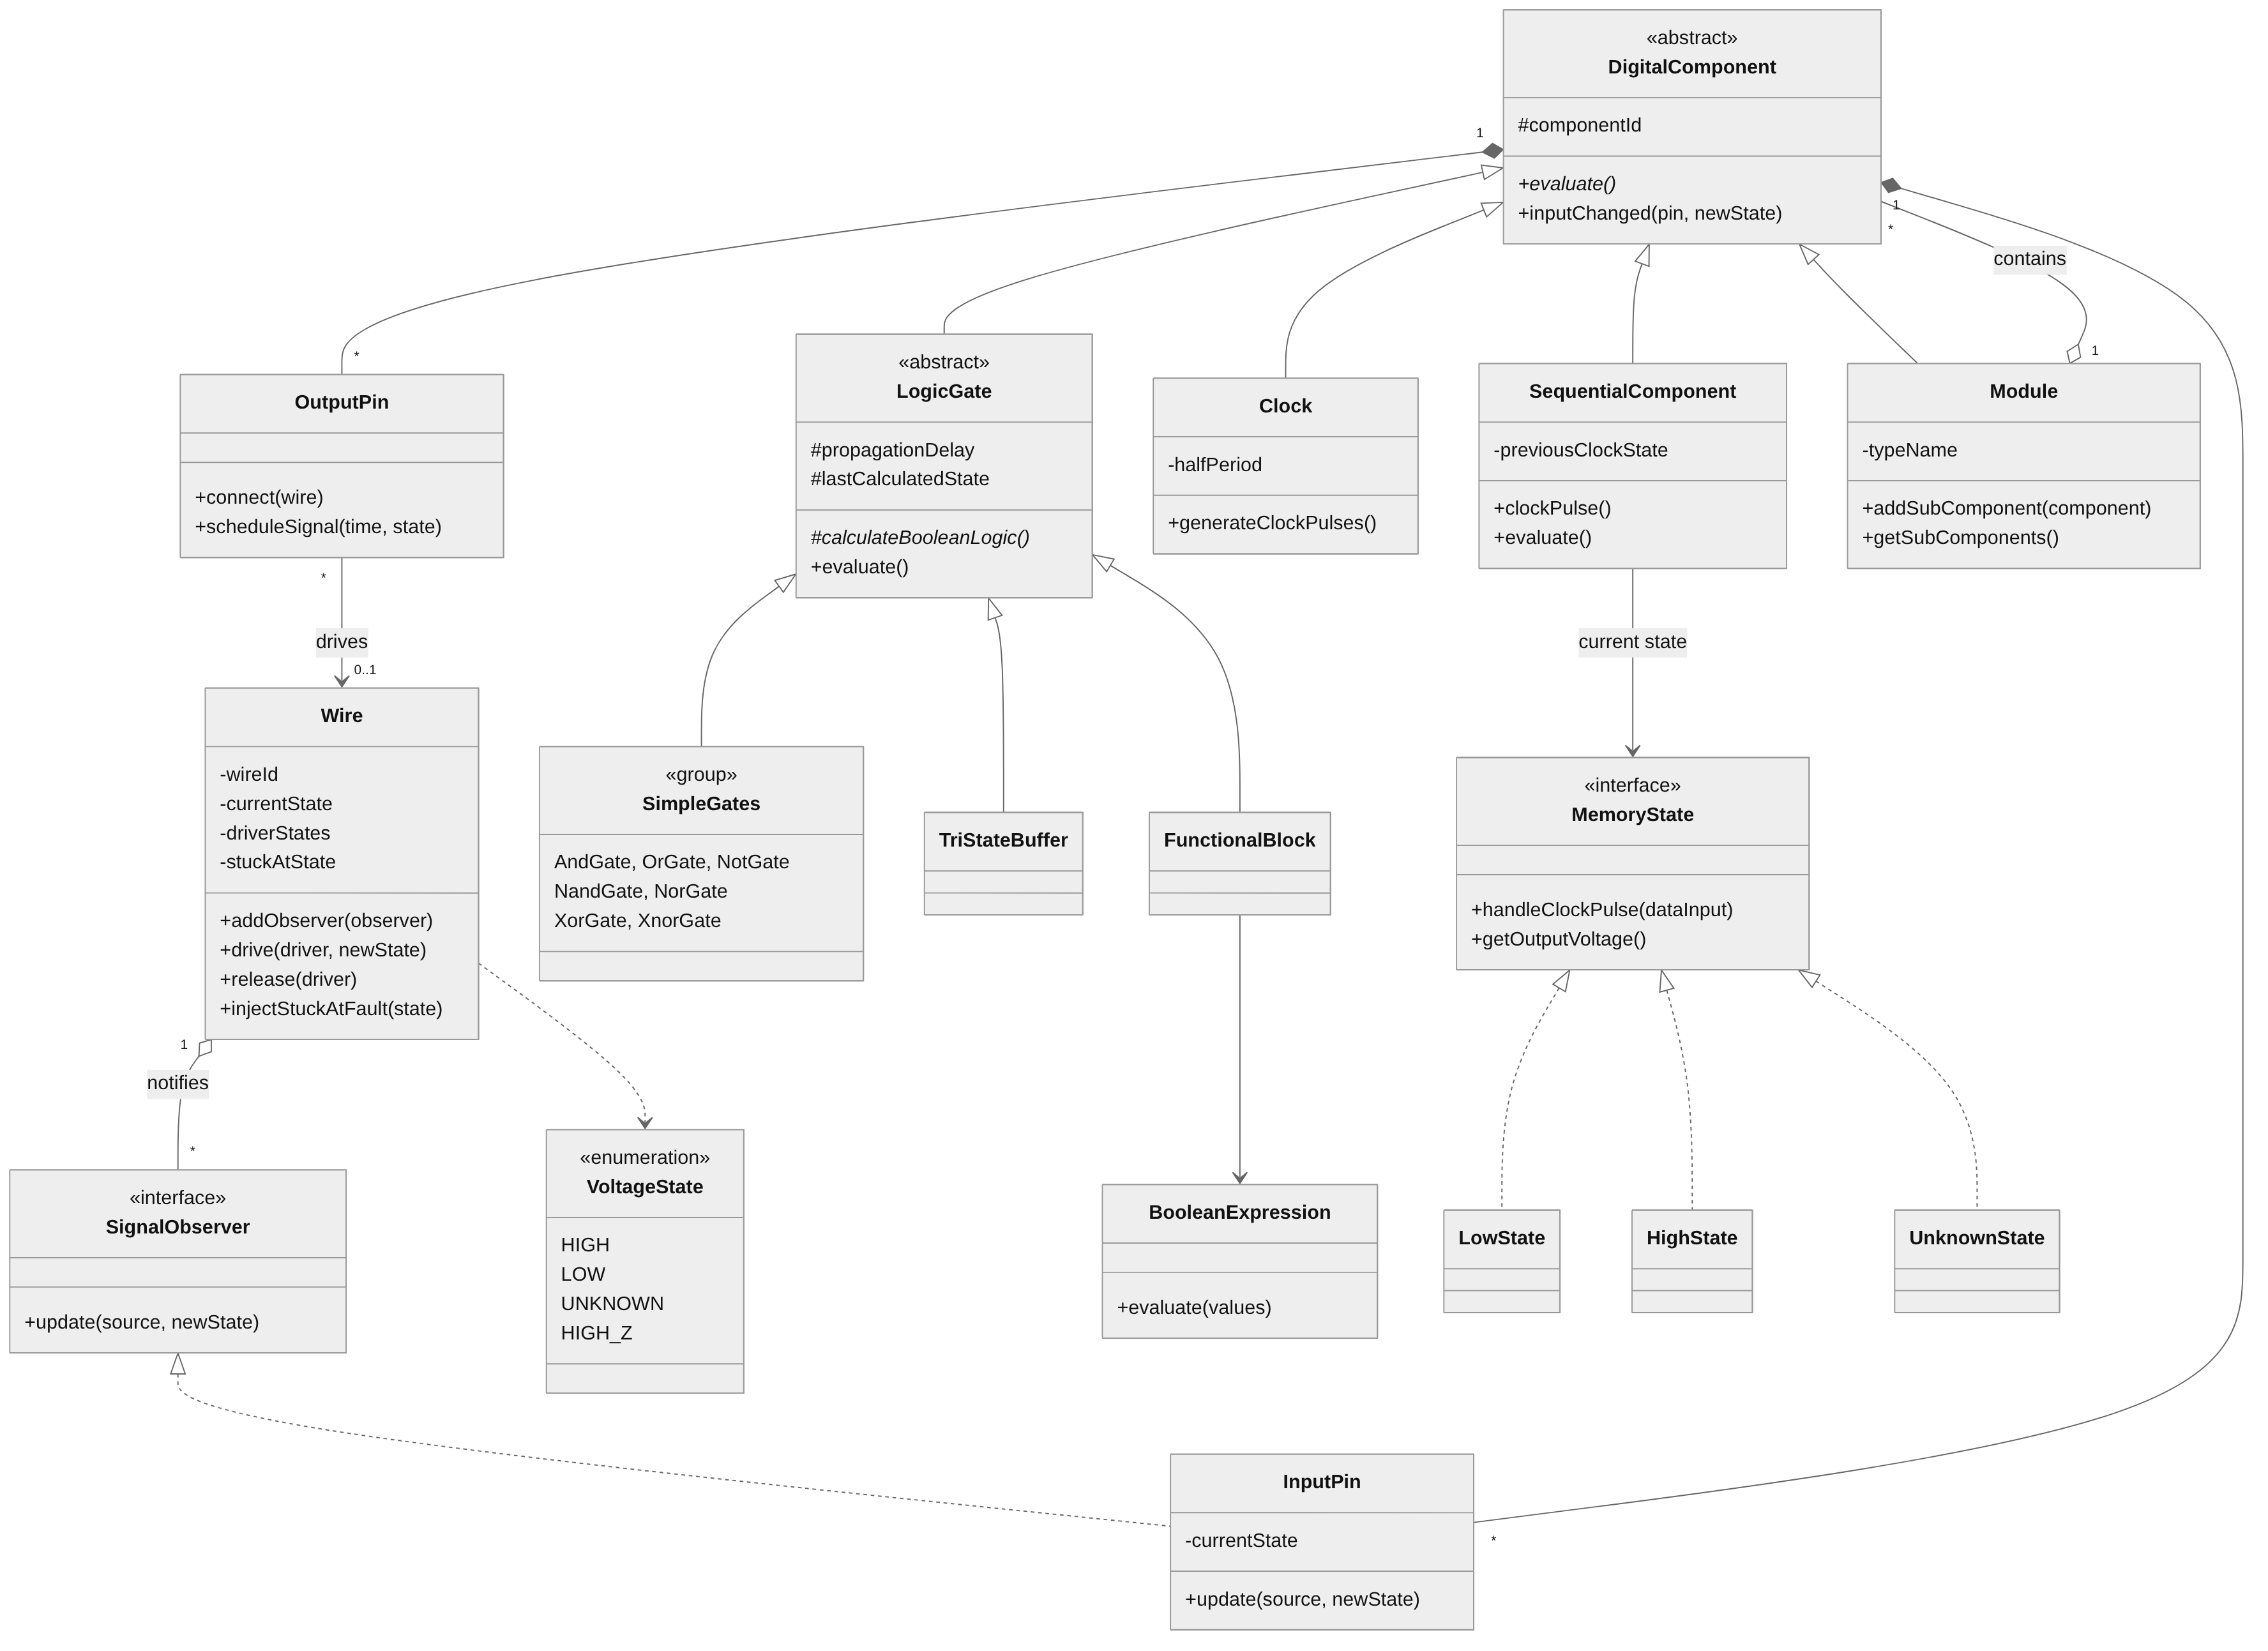
\includegraphics[width=\textwidth]{classDiagramDomain.png}
\caption{Class diagram of the domain model}
\label{fig:classdomain}
\end{figure}

Figure~\ref{fig:classengine} presents the parsing, engine, and analysis classes.
\texttt{SimulationRunner} coordinates a single simulation run.
\texttt{SimulationContext} owns the \texttt{EventEngine} and the assertions of that run.
The analysis classes create their own contexts, so their internal simulations remain separate from each other.

\begin{figure}[H]
\centering
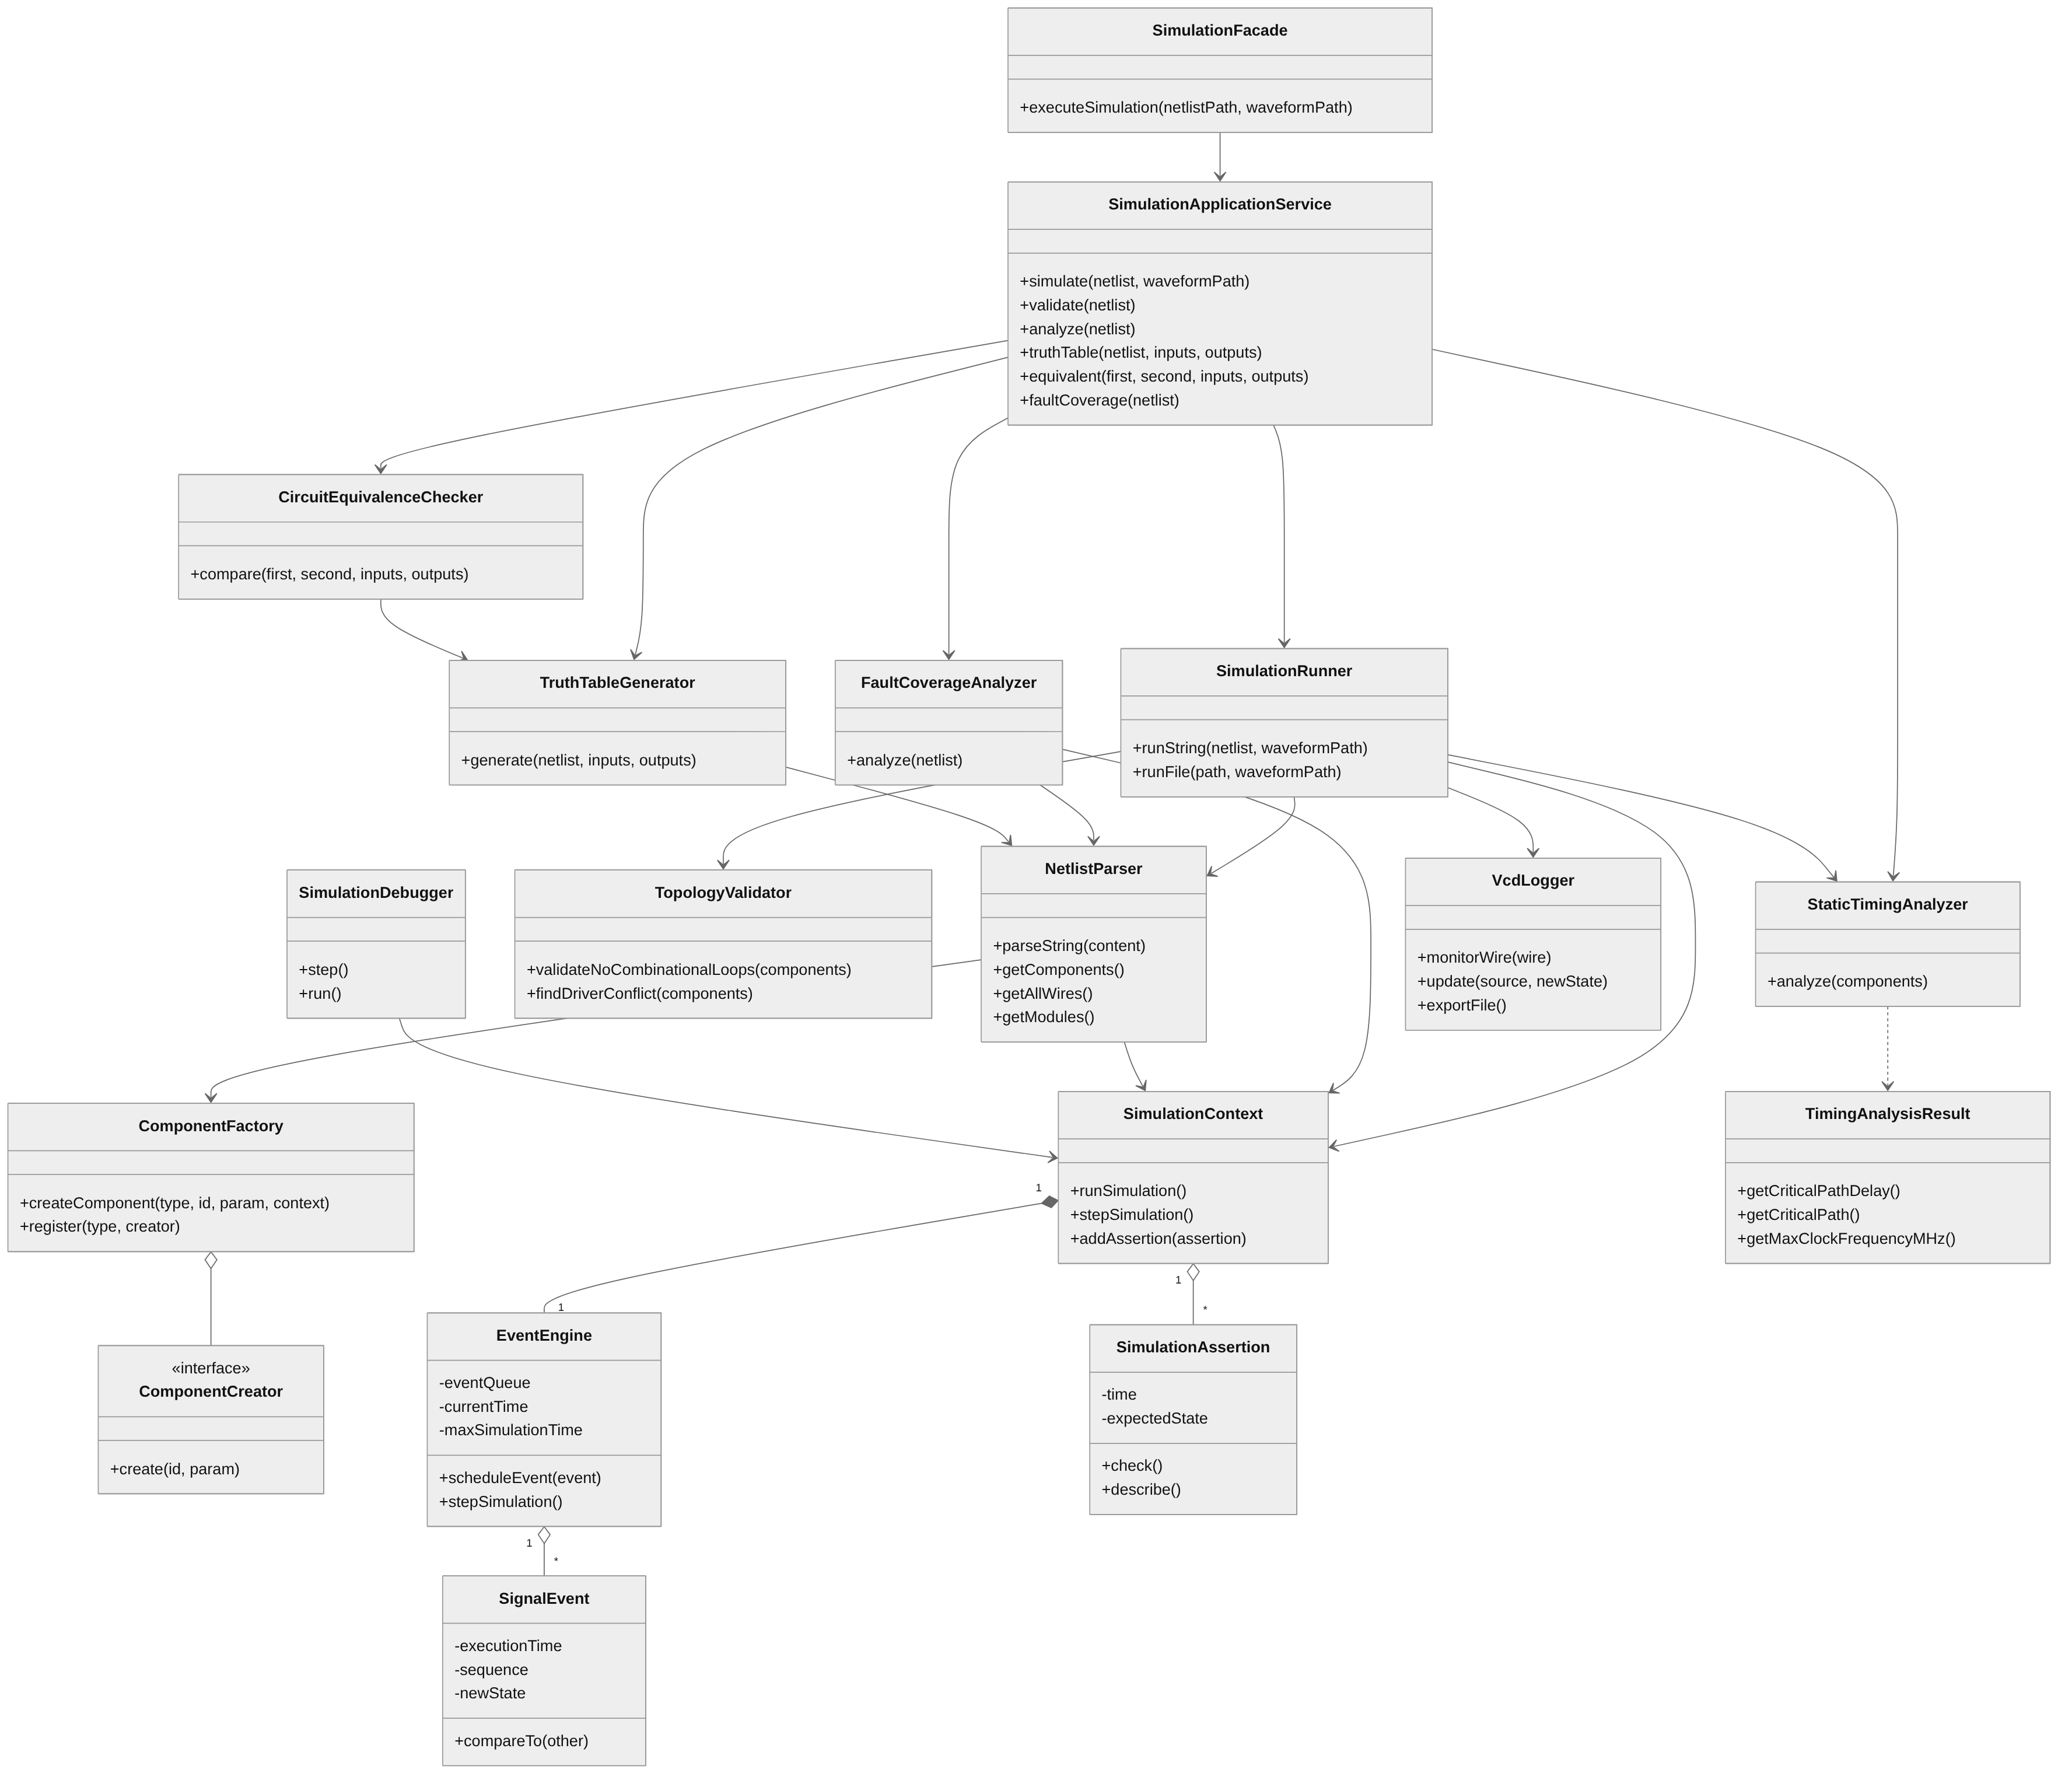
\includegraphics[width=\textwidth]{classDiagramEngine.png}
\caption{Class diagram of the parsing, engine, and analysis classes}
\label{fig:classengine}
\end{figure}

\subsection{Interaction Model}

Figure~\ref{fig:seqrun} presents the messages of one simulation run.
The user interface passes the netlist to the service, and \texttt{SimulationRunner} carries out the phases of the pipeline in order.

\begin{figure}[H]
\centering
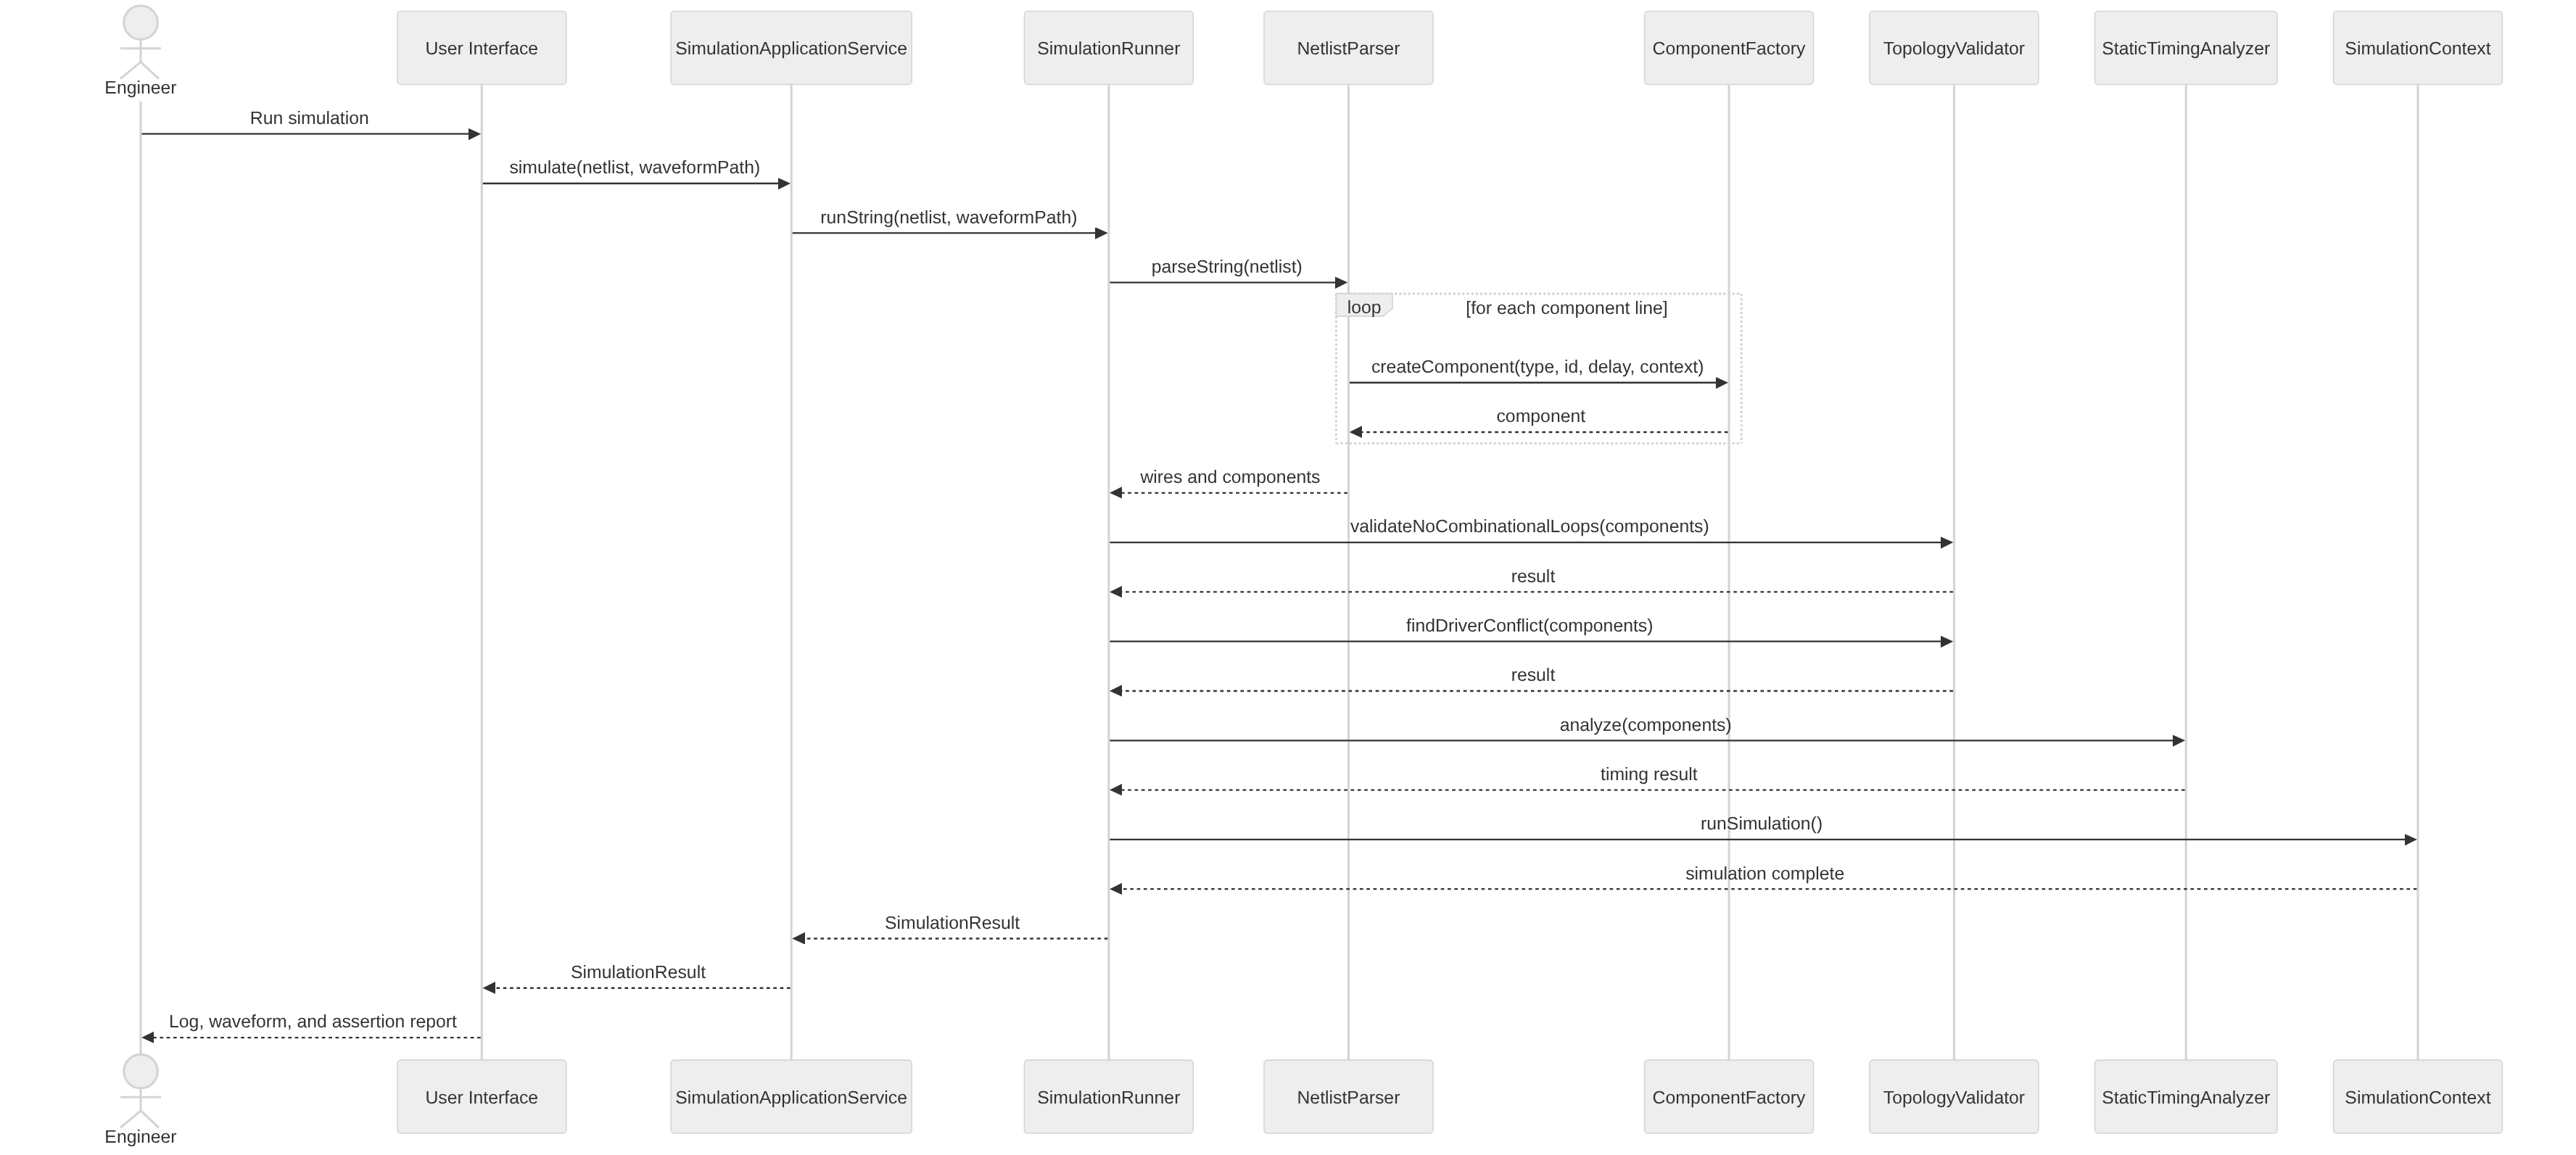
\includegraphics[width=\textwidth]{sequenceDiagramRun.png}
\caption{Sequence diagram of a simulation run}
\label{fig:seqrun}
\end{figure}

Figure~\ref{fig:seqevent} presents the processing of one event.
The queue orders events by time and then by creation order, so a given netlist always produces the same result.
A gate schedules a new event only when its calculated output changes.
The engine therefore avoids work for signals that have no effect.

\begin{figure}[H]
\centering
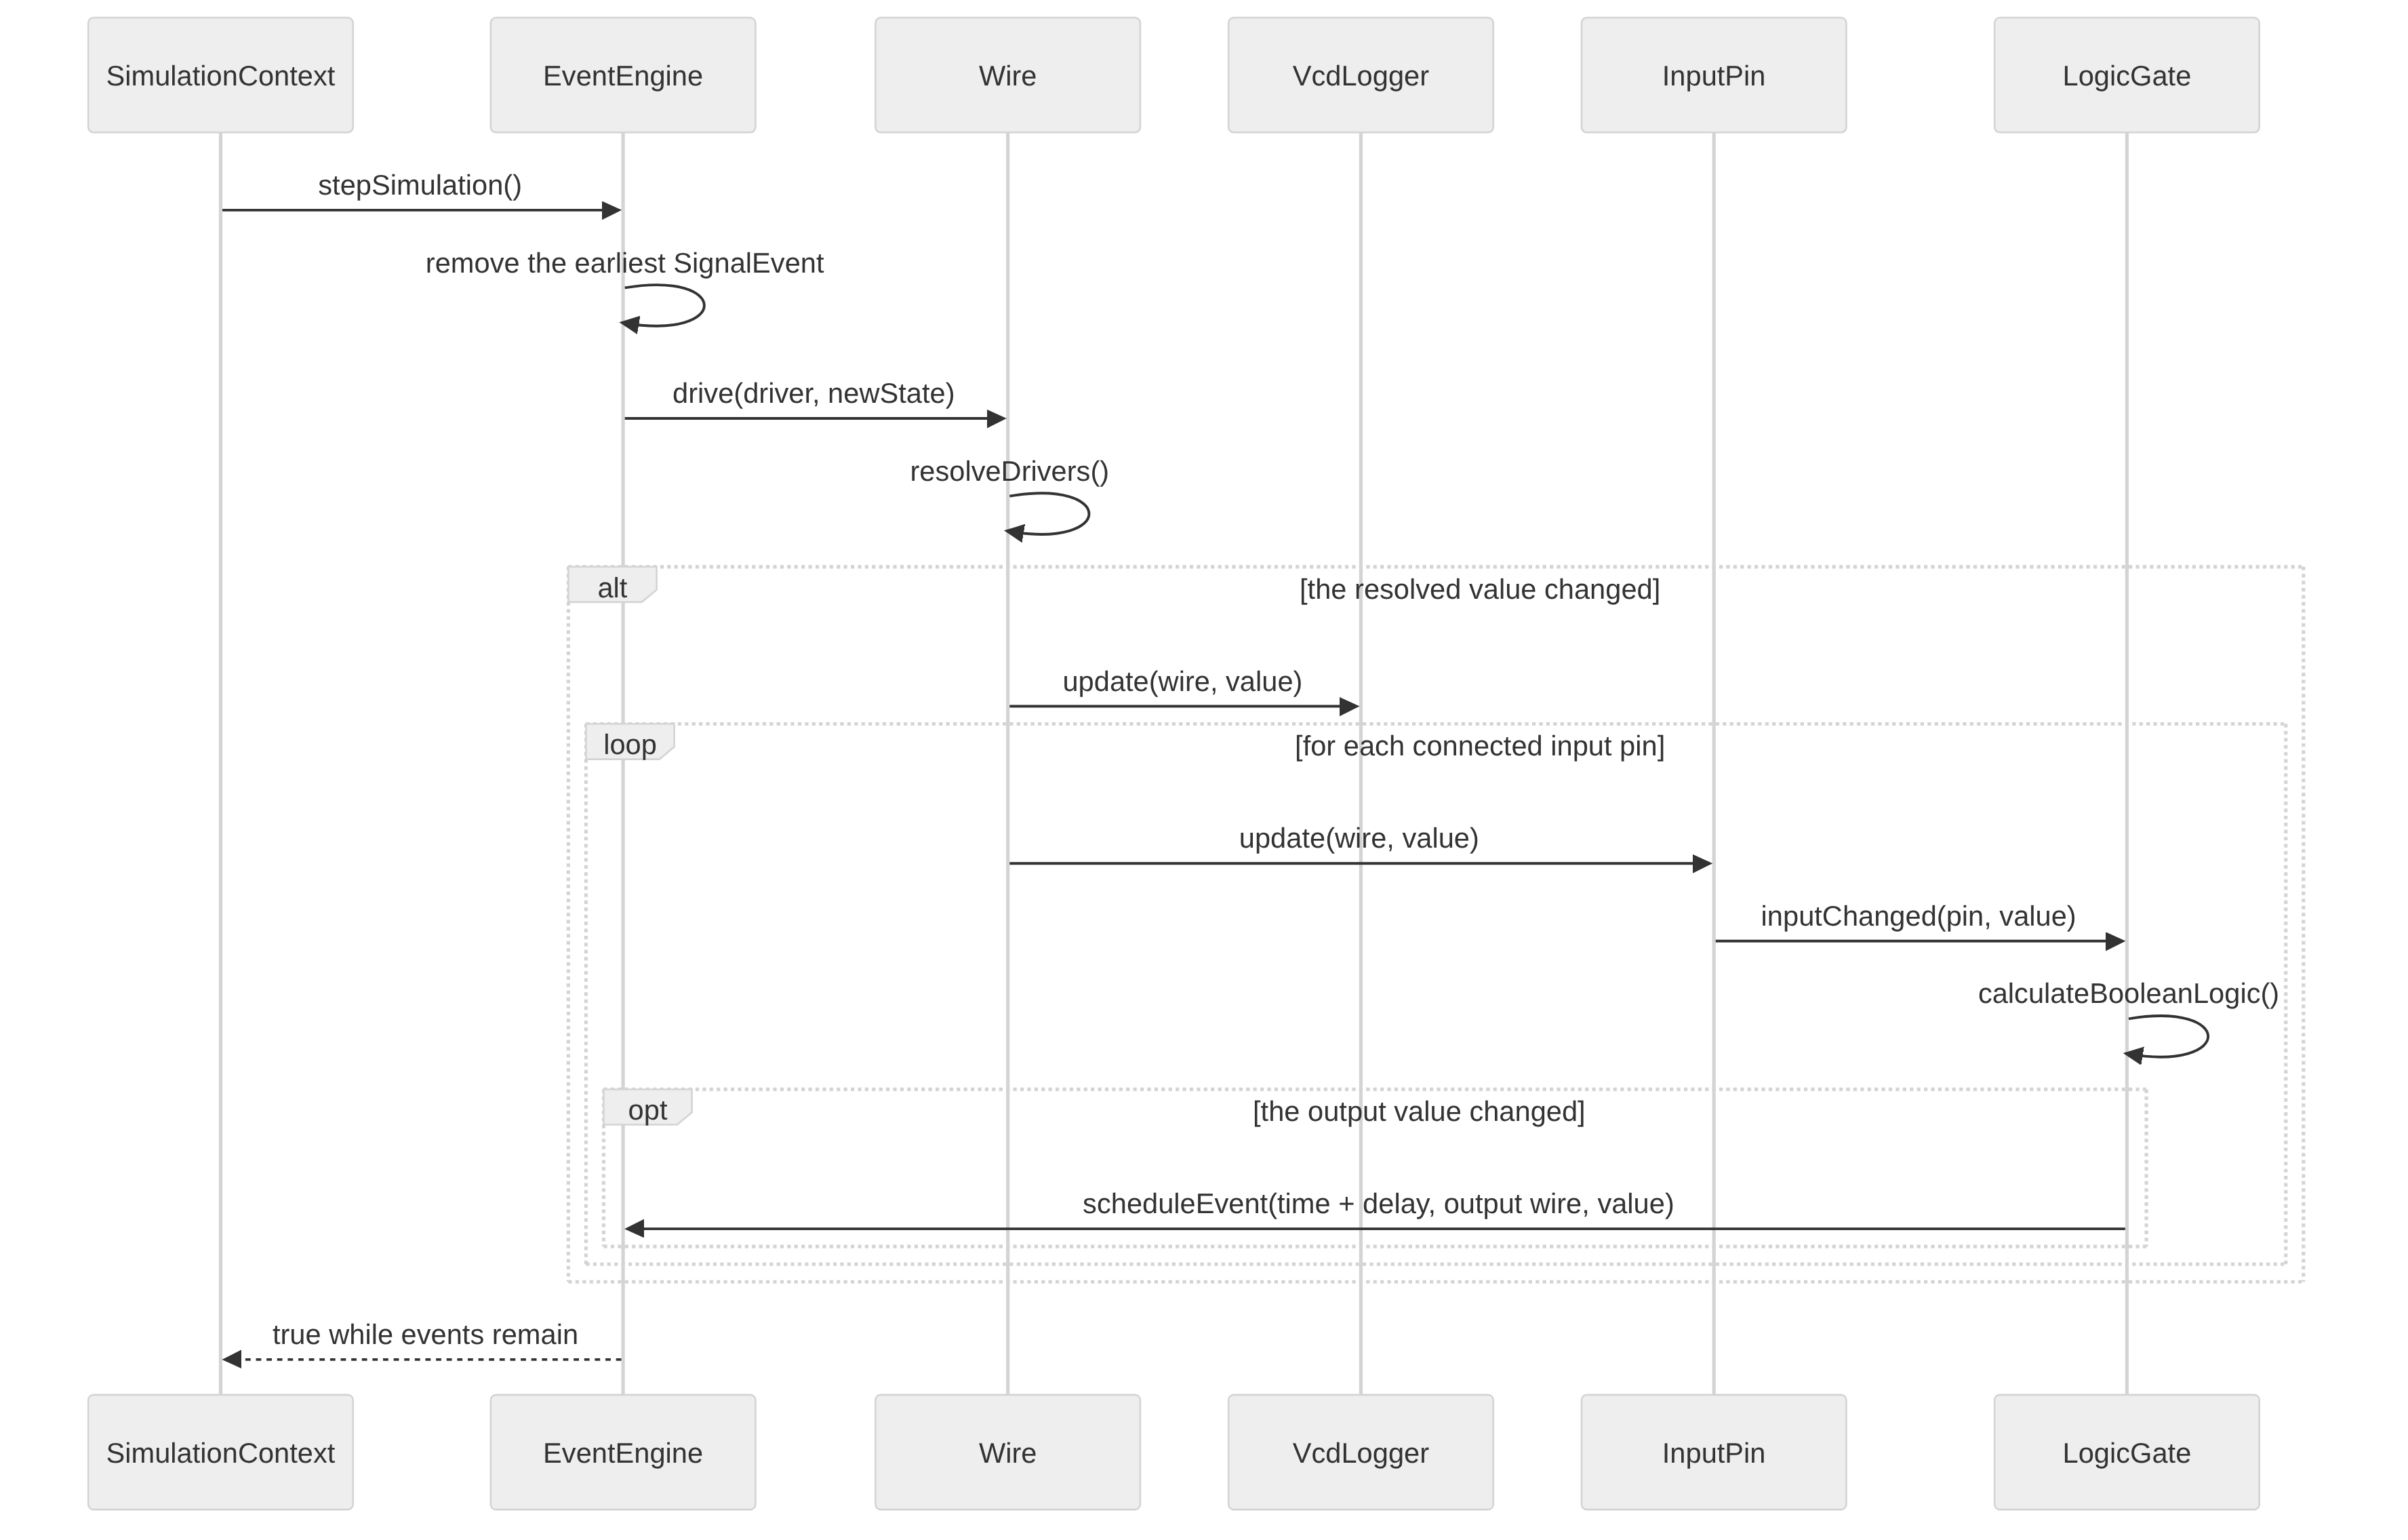
\includegraphics[width=\textwidth]{sequenceDiagramEvent.png}
\caption{Sequence diagram of the processing of one event}
\label{fig:seqevent}
\end{figure}

A wire resolves the values of its drivers on each update.
The wire takes the value X when one driver holds X or when two drivers disagree.
It takes the value Z when every driver has released it.
It takes the common value when the remaining drivers agree.
A stuck-at fault overrides all drivers until the end of the run.

\subsection{State Model}

Figure~\ref{fig:state} presents the states of a flip-flop.
A flip-flop starts in \texttt{LowState} and changes state only on a rising clock edge.
A data input of X or Z moves it to \texttt{UnknownState}, and the next known data value restores a known state.
The transitions that keep a flip-flop in its present state do not appear in the figure.

\begin{figure}[H]
\centering
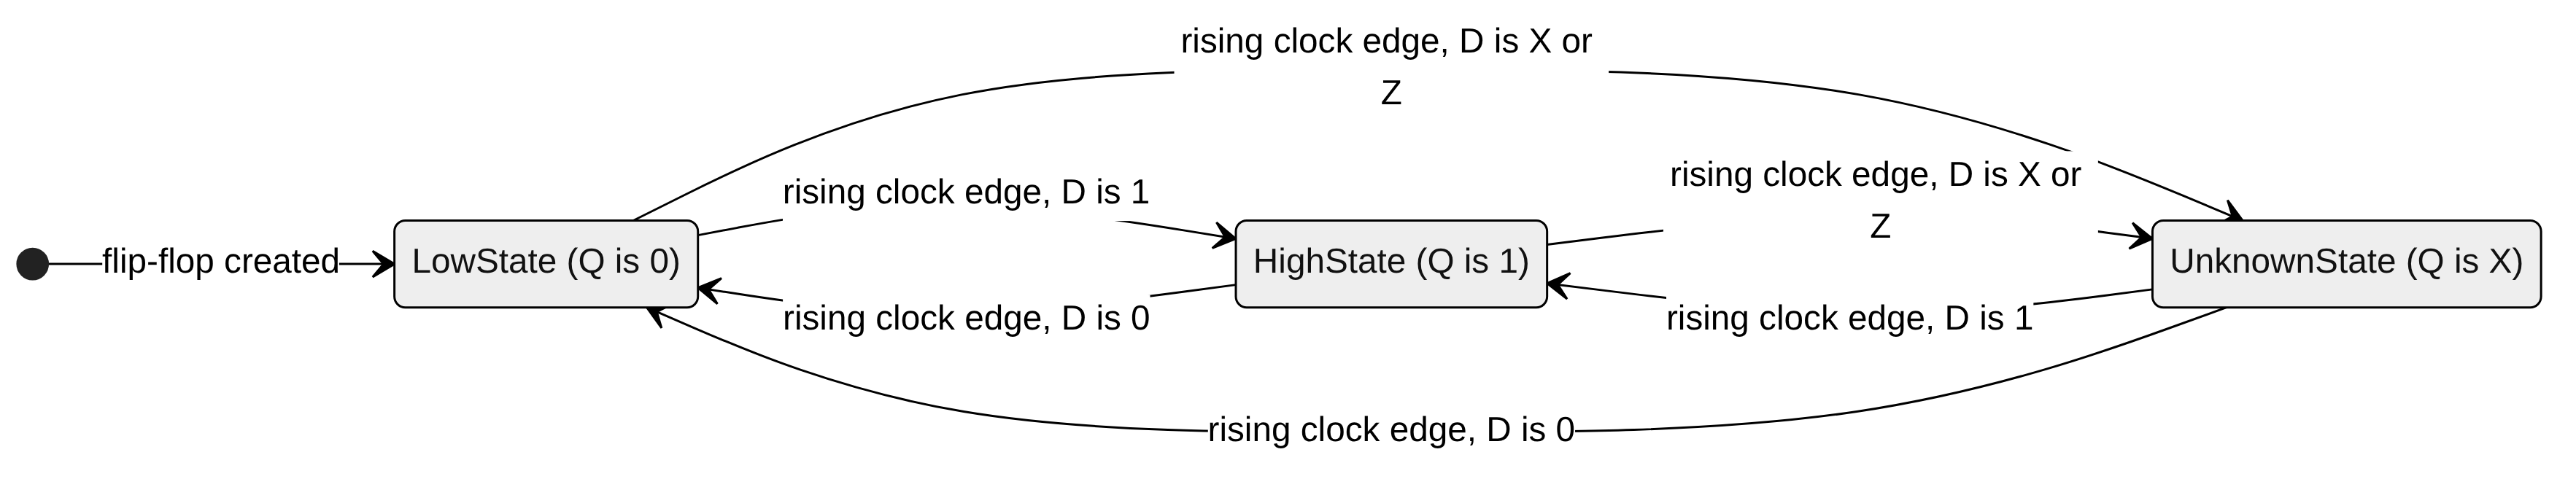
\includegraphics[width=\textwidth]{stateDiagramMemory.png}
\caption{State diagram of a flip-flop}
\label{fig:state}
\end{figure}

\subsection{Netlist Language}

A netlist is a plain text file with one command on each line.
Figure~\ref{fig:netlist} presents a half adder that uses the language.
The \texttt{SIM\_TIME} command sets the duration, and \texttt{WIRE} declares a wire.
Each gate line gives the gate type, a name, a delay in nanoseconds, the input wires, and the output wire.
\texttt{STIMULUS} sets an input at a given time, and \texttt{ASSERT} checks a wire at a given time.
The language also provides macros through \texttt{DEF} and \texttt{ENDDEF}, Boolean functions through \texttt{FUNC}, faults through \texttt{FAULT}, and a library of adders, multiplexers, and decoders.

\begin{figure}[H]
\centering
\begin{lstlisting}
# Half adder
SIM_TIME 100

WIRE A
WIRE B
WIRE Sum
WIRE Carry

XOR sum_gate 10 A B Sum
AND carry_gate 10 A B Carry

STIMULUS 0 A 1
STIMULUS 0 B 1

ASSERT 50 Sum 0
ASSERT 50 Carry 1
\end{lstlisting}
\caption{Netlist of a half adder with stimuli and assertions}
\label{fig:netlist}
\end{figure}

\subsection{Analysis Algorithms}

\textbf{Static timing analysis.}
The analyzer finds the slowest route through the components with a memoized depth-first search.
A route may start at a flip-flop, whose own delay represents its clock-to-output time, and it ends at the data input of the next flip-flop.
The maximum clock frequency is the inverse of the critical path delay.

\textbf{Truth tables and state tables.}
The generator builds a fresh circuit for each input combination, applies the inputs, and runs the simulation until no event remains.
For a sequential circuit, it also forces each combination of stored values and reads the next state from the data inputs of the flip-flops.
This table includes the internal variables, as the reference paper proposes for sequential circuits \refDezan{}.

\textbf{Equivalence checking.}
The checker generates the tables of two circuits and compares them row by row, following the method of the reference paper \refDezan{}.
It reports the first row that differs.

\textbf{Fault coverage.}
The analyzer simulates the circuit once without a fault.
It then repeats the simulation once for each wire stuck at 0 and once for each wire stuck at 1.
A fault counts as detected when an output or a flip-flop holds a known value that differs from the fault-free value at some time.

\textbf{Schematic layout.}
The layout places components in columns by signal flow, which follows the layered drawing method of Sugiyama, Tagawa, and Toda \refSugiyama{}.
It orders the components in each column to reduce wire crossings, and it routes wires through tracks between the columns.

\subsection{User Interfaces}

The desktop application, built with Java Swing, provides an editor beside tabs for the log, waveform, schematic, analysis, and user guide.
Figure~\ref{fig:desktop} presents the waveform tab with the two-bit counter from the sample set.
Figure~\ref{fig:schematic} presents the schematic tab with a two-bit adder built from macros.
The highlighted route in this figure is the critical path, and a time slider colors each wire by its value.

\begin{figure}[H]
\centering
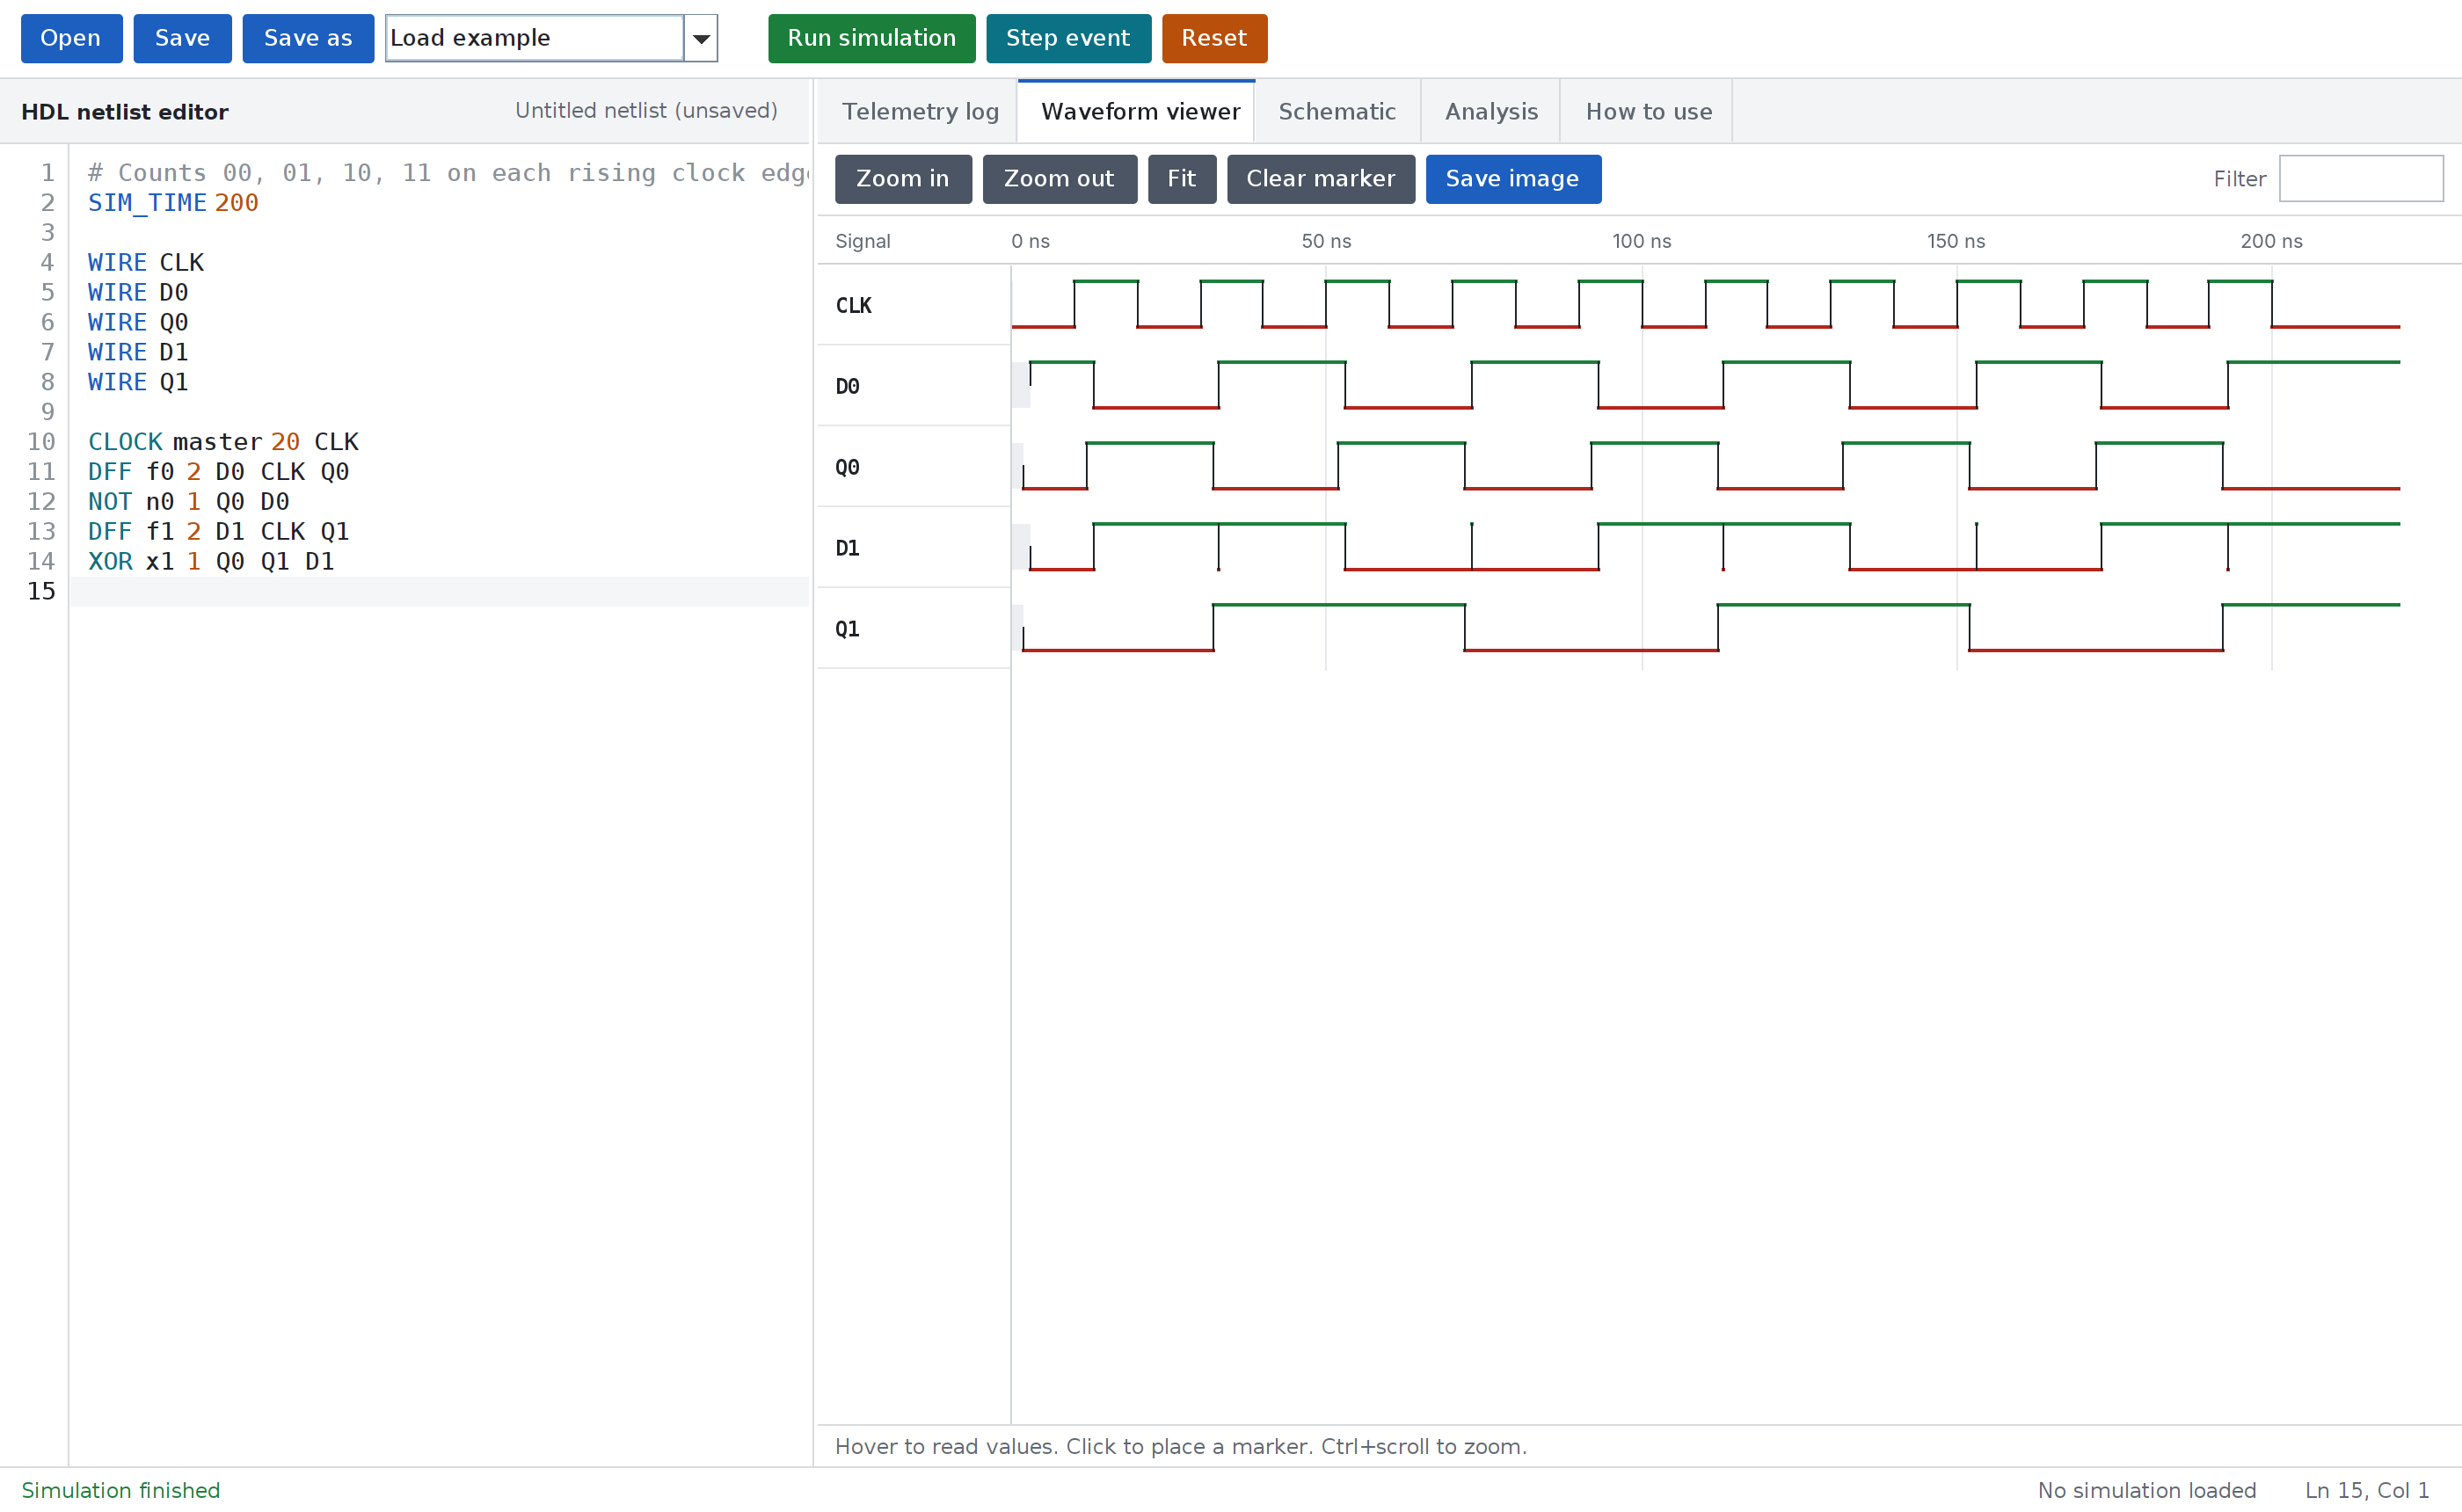
\includegraphics[width=\textwidth]{desktop-waveform.png}
\caption{Waveform tab of the desktop application}
\label{fig:desktop}
\end{figure}

\begin{figure}[H]
\centering
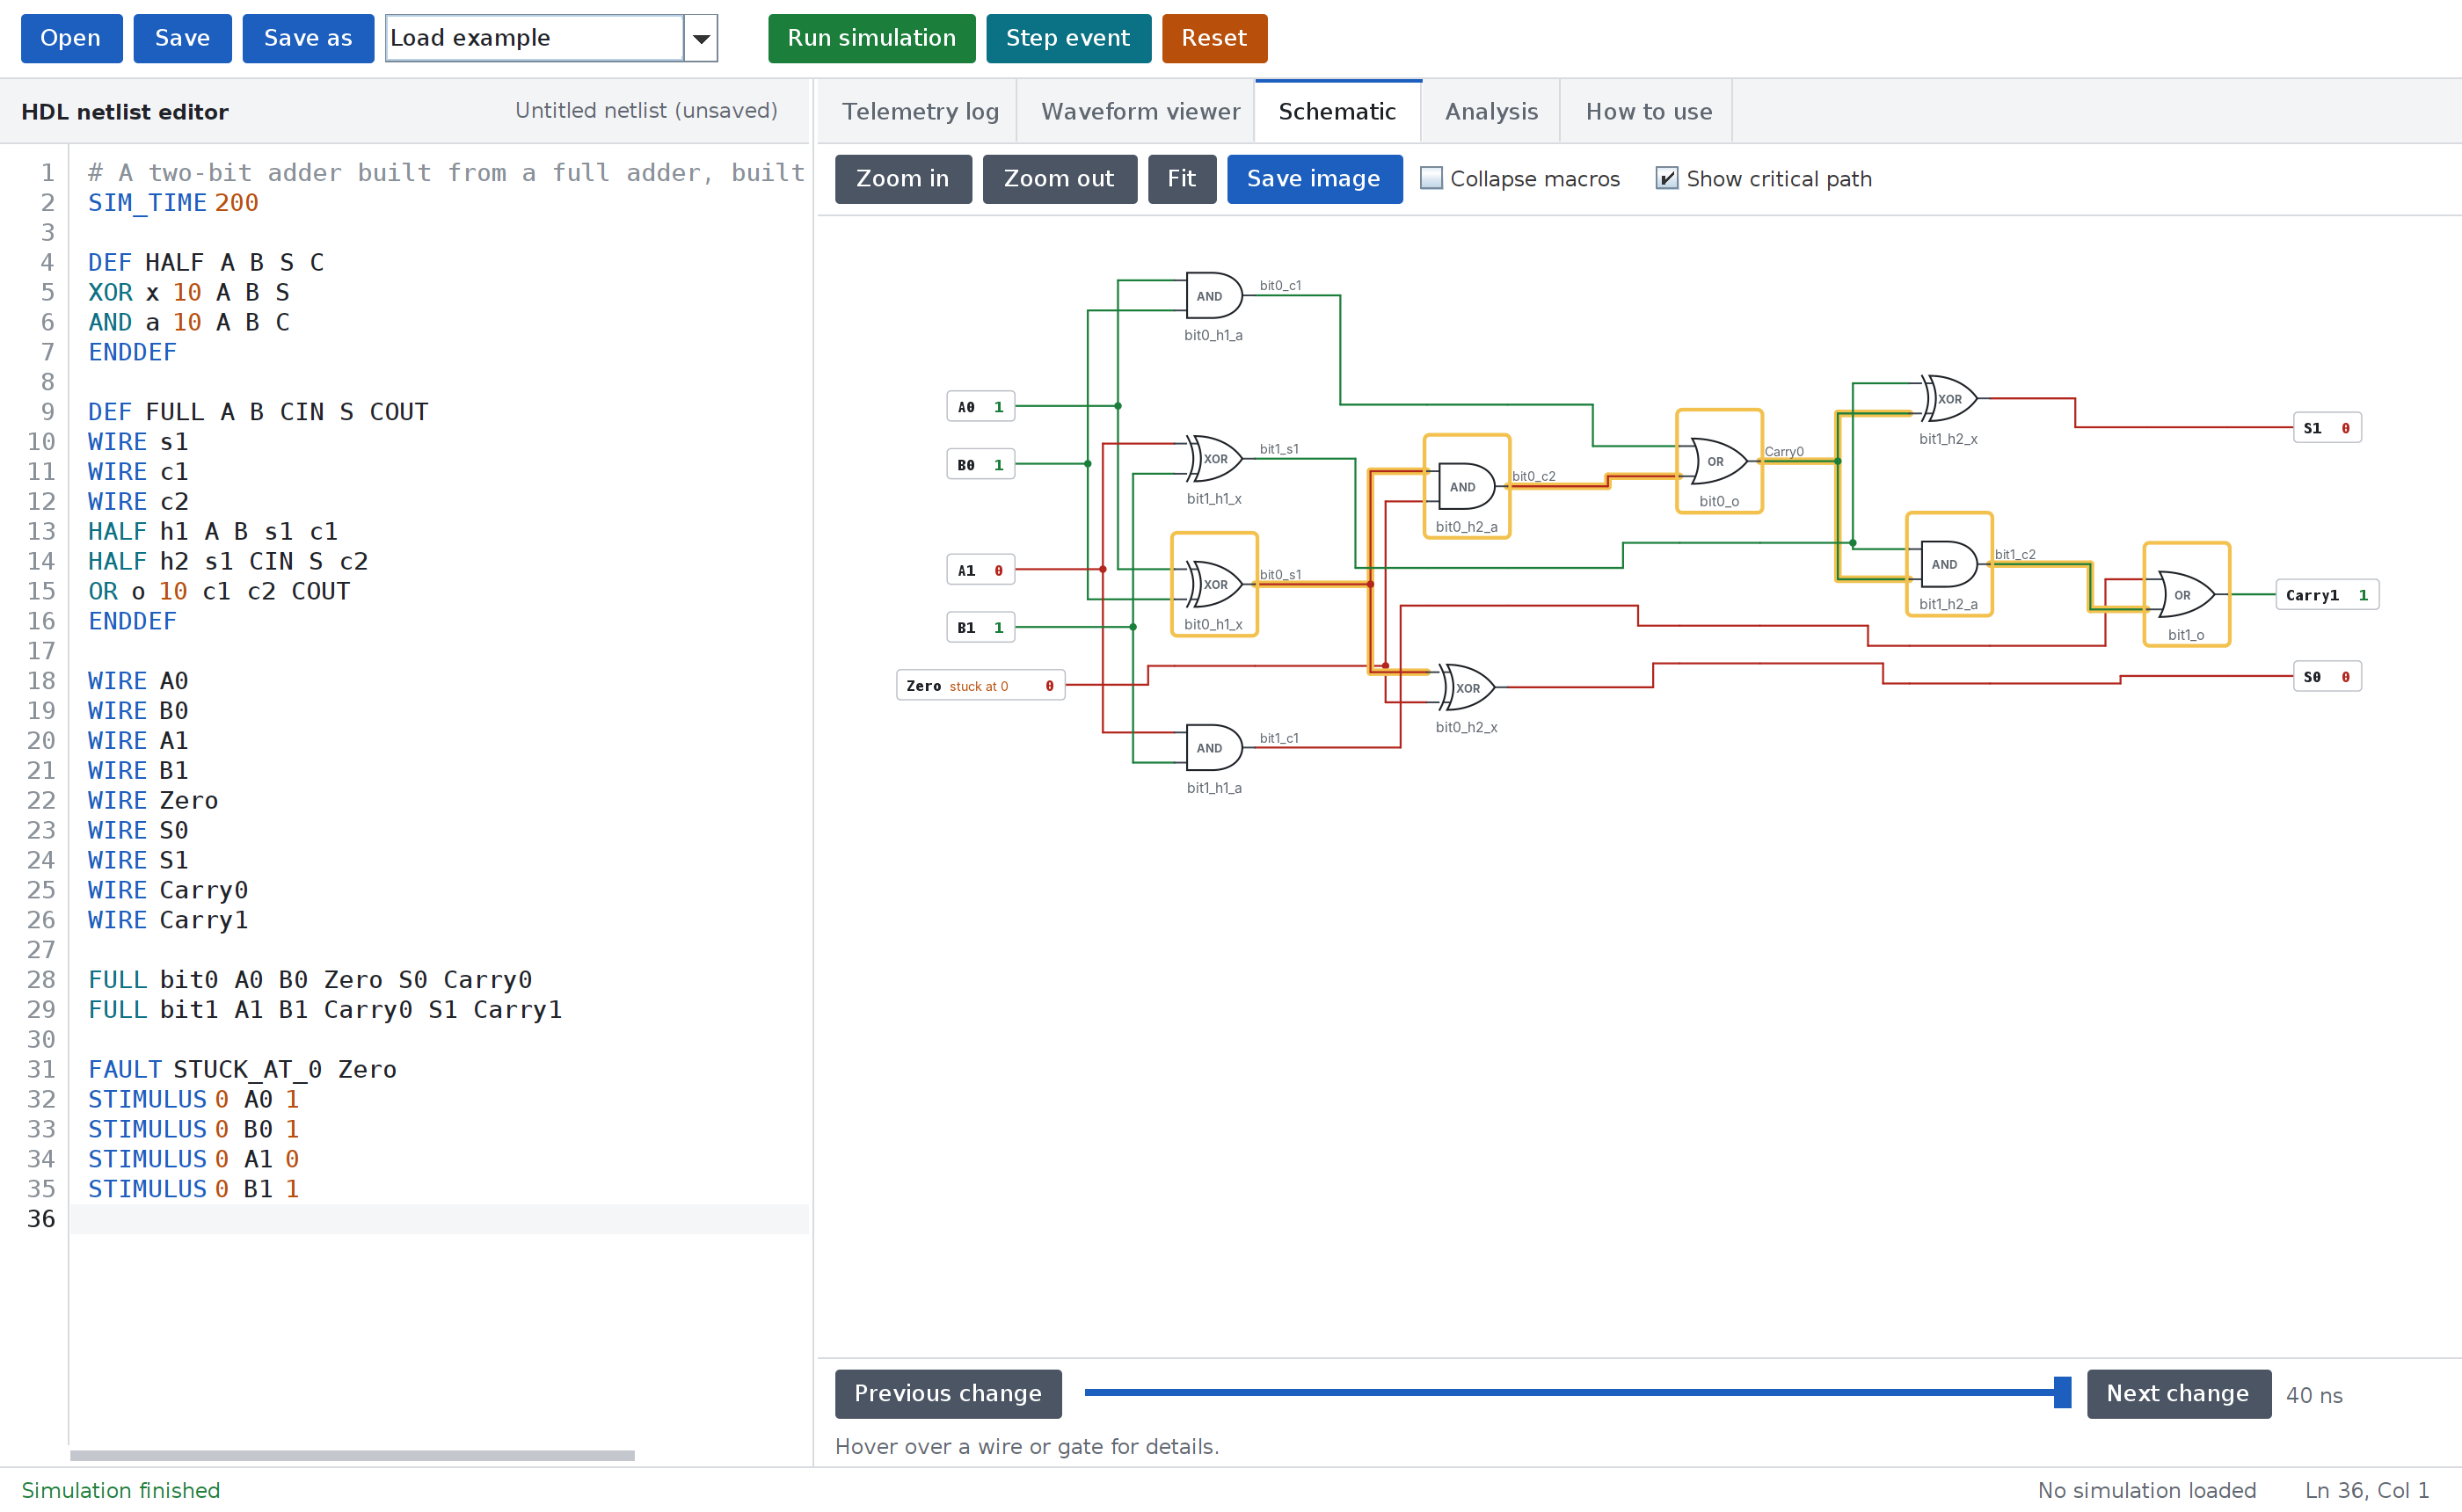
\includegraphics[width=\textwidth]{desktop-schematic.png}
\caption{Schematic tab with the critical path highlighted}
\label{fig:schematic}
\end{figure}

The hosted browser version \refHosted{} offers the same tabs and the same results.
The command line tool exposes each operation as a command with an exit status, so scripts can use it for automated checks.
Exported VCD files open in external viewers such as GTKWave \refGTKWave{}.

\section{Implementation and Evaluation}
\label{sec:evaluation}
\subsection{Implementation Environment}
\subsection{Sample Circuits and Results}
\subsection{Test Coverage}
\subsection{Comparison with the Reference Paper}
\subsection{Known Limitations}
\label{sec:limitations}

\section{Summary and Conclusion}
\label{sec:conclusion}

This project set out to implement the object-oriented circuit models of Dezan, Lagadec, and Pottier \refDezan{} and to extend them with timing and fault analysis.
The resulting Java system simulates combinational, sequential, and hierarchical circuits from text netlists.
It adds a discrete-event engine, static timing analysis, fault coverage, and assertions.
A desktop application, a command line tool, and a browser application all use the same engine.

The evaluation supports three observations.
First, the sample results agree with the expected behavior of the circuits, including their truth tables and state tables.
Second, the JUnit suite covers 91.3 percent of the source lines outside the desktop interface.
The engine also processed more than one million events per second in the measured configuration.
Third, Dependency Injection keeps repeated simulation runs independent, and truth table generation and fault coverage rely on this property.

Two requirements remain only partly met.
A new gate type needs one registration call in addition to its class, and the engine simulates expanded gates in place of modules.
The largest gap with the reference paper is the absence of integer signal values and FPGA support.

Future work could add multi-bit buses and integer truth tables.
It could also let the engine evaluate modules directly and extend timing analysis with setup and hold times.
These extensions would bring the system closer to the mixed-level model that the reference paper proposes.

\section*{References}
\addcontentsline{toc}{section}{References}
\sloppy

\printreferences

\section*{Internet Sources}
\addcontentsline{toc}{section}{Internet Sources}

\printinternetsources


\end{document}
